%
%   Prof. Dr. Julian Reichwald
%   auf Basis einer Vorlage von Prof. Dr. Jörg Baumgart
%   DHBW Mannheim
%
%	ACHTUNG: Für das Erstellen des Literaturverzeichnisses wird das modernere Paket biblatex
%			 in Kombination mit biber verwendet -- nicht mehr das ältere BibTex!
% 			 Bitte stellen Sie ggf. Ihre TeX-Umgebung
% 			 entsprechend ein (z.B. TeXStudio: Einstellungen --> Erzeugen --> Standard Bibliographieprogramm: biber)
%

\documentclass[
	12pt,
	BCOR=5mm,
	DIV=12,
	headinclude=on,
	footinclude=off,
	parskip=half,
	bibliography=totoc,
	listof=entryprefix,
	toc=listof,
	number=noenddot,
	plainfootsepline]{scrreprt}

%	Konfigurationsdatei einbinden
% !TEX root = ../master.tex

%-------------------
% 		HYPERREF
%-------------------

\PassOptionsToPackage{hyphens}{url}\usepackage[hidelinks=true]{hyperref}
 % hidelinks=true verhindert rote Ränder bei Links im Dokument.
 
 \newcommand{\urlinline}[1]{(\textsf{\footnotesize{\url{{#1}}}})}

% Zwei eigene Befehle zum Setzen von Autor und Titel. Ausserdem werden die PDF-Informationen richtig gesetzt.
\newcommand{\titel}[1]{\def\dertitel{#1}\hypersetup{pdftitle={#1}}}
\newcommand{\autor}[1]{\def\derautor{#1}\hypersetup{pdfauthor={#1}}}

%-----------------------------------
%		SCHRIFT UND ENCODING
%-----------------------------------
\usepackage[T1]{fontenc}
\usepackage[utf8]{inputenc}

\usepackage{setspace}
%\onehalfspacing
%TODO use this spacing

%---------------------------
%		BERECHNUNGEN
%---------------------------
\usepackage{calc} % Used for extra space below footsepline

%---------------------------------
%		SPRACHEINSTELLUNGEN
%---------------------------------
% Voreinstellungen für Deutsch und Englisch. Die nicht verwendete Sprache ist auszukommentieren.
% DEUTSCH
%\usepackage[ngerman]{babel}
%\usepackage[german=quotes]{csquotes}

%ENGLISCH
\usepackage[english]{babel}
\usepackage{csquotes} % Richtiges Setzen der Anführungszeichen mit \enquote{}

%----------------------------
%		BIBLIOGRAFIE
%----------------------------
% Voreinstellungen für Fußnotenzitate (Autor-Jahr), IEEE-Standard, Alphabetic-Stil und Havard-Stil. Die nicht verwendeten Stile müssen auskommentiert werden

% \usepackage[backend=biber, autocite=footnote, style=authoryear, dashed=false]{biblatex}		% Fußnotenzitate
% \usepackage[backend=biber, autocite=inline, style=ieee]{biblatex}							% IEEE-Stil
% \usepackage[backend=biber, autocite=inline, style=alphabetic]{biblatex}					% Alphabetic-Stil
% \usepackage[backend=biber, autocite=inline, style=authoryear, dashed=false]{biblatex}		% Harvard-Stil
\usepackage[backend=biber, autocite=inline, style=apa]{biblatex}							% APA-Stil

% Fußnotenzitate mit YYYY-MM-DD in Bibliographie
% \usepackage[backend=biber, autocite=footnote, style=authoryear, dashed=false, urldate=edtf, date=edtf, seconds=true]{biblatex}

% Zum Zählen der Fußnoten über Kapitel hinaus
\usepackage{chngcntr}
\counterwithout{footnote}{chapter}

\DefineBibliographyStrings{ngerman}{  %Change u.a. to et al. (german only!)
	andothers = {{et\,al\adddot}},
}

\setlength{\bibparsep}{\parskip}		%add some space between biblatex entries in the bibliography
\addbibresource{adds/bibliography.bib}	%Add file bibliography.bib as biblatex resource

%----------------------
%		ACRONYME
%----------------------
%%%
%%% WICHTIG: Installieren Sie das neueste Acronyms-Paket!!!
%%%
\makeatletter
\usepackage[printonlyused]{acronym}
\@ifpackagelater{acronym}{2015/03/20}
  {%
    \renewcommand*{\aclabelfont}[1]{\textbf{\textsf{\acsfont{#1}}}}
  }%
  {%
  }%
\makeatother

%--------------------
%		GLOSSAR
%--------------------
%\usepackage[toc]{glossaries}					% für Seitenreferenzen im Glossar
\usepackage[toc, nonumberlist]{glossaries}		% ohne Seitenreferenzen im Glossar

%---------------------
%		LISTINGS
%---------------------
\usepackage{listings}
% Listings formatieren
%\renewcommand{\lstlistlistingname}{Quelltextverzeichnis}
\lstset{numbers=left,
	numberstyle=\tiny,
	captionpos=b,
	breaklines=true,
	basicstyle=\linespread{0.8}\ttfamily\small}

%-------------------------------
%		ZUSÄTZLICHE PAKETE
%-------------------------------
\usepackage{lipsum}				% Blindtext
\setlipsumdefault{1-4}
\usepackage[pdftex]{graphicx} 			% verschiene Bildformate einbinden
\usepackage{pdfpages}		% PDF einbinden
\usepackage{varioref} 	% schönere Referenzen über \vref{}
\usepackage{caption}			% schönere Überschriften
\usepackage{booktabs}			% bessere Tabs
\usepackage{array}
\newcolumntype{P}[1]{>{\raggedright\arraybackslash}p{#1}}

%--------------------------
%		Tikz diagram library
%--------------------------
\usepackage{tikz}
\usetikzlibrary{arrows,decorations.pathmorphing,backgrounds,fit,positioning,shapes.symbols,chains}

%--------------------------
%		TpX used packages
%--------------------------
\usepackage{color}
\DeclareGraphicsExtensions{.pdf,.png,.jpg,.jpeg,.mps}
\usepackage{pgf}
\usepackage{epic,bez123}
\usepackage{floatflt}% package for floatingfigure environment
\usepackage{wrapfig}% package for wrapfigure environment

%-------------------------
%		ALGORITHMEN
%-------------------------
\usepackage{algorithm}
\usepackage{algpseudocode}
\renewcommand{\listalgorithmname}{List of algorithms}
\floatname{algorithm}{algorithm}

%-------------------------
%		SCHRIFTART
%-------------------------
% Entweder Latin Modern oder Times / Helvetica
\usepackage{lmodern} %Latin modern font
%\usepackage{mathptmx}  %Helvetica / Times New Roman fonts (2 lines)
%\usepackage[scaled=.92]{helvet} %Helvetica / Times New Roman fonts (2 lines)

%------------------------------------
%		KOPFZEILE / FUßZEILE
%------------------------------------
%	   ACHTUNG! Einige einstellungen werden in master.tex erneut verändert
\RequirePackage[automark,headsepline,footsepline]{scrpage2}
\pagestyle{scrheadings}
\renewcommand*{\pnumfont}{\upshape\sffamily}
\renewcommand*{\headfont}{\upshape\sffamily}
\renewcommand*{\footfont}{\upshape\sffamily}
\renewcommand{\chaptermarkformat}{}

\clearscrheadfoot

% using cfoot centers the header 
% use ofoot for outer side, especially with documentclass[twoside]
\cfoot[\rule{0pt}{\ht\strutbox+\dp\strutbox}\pagemark]{\rule{0pt}{\ht\strutbox+\dp\strutbox}\pagemark}

\ohead{\headmark}

%TODO: fix footer

%-----------------------------------
%		Fix Headheight
%-----------------------------------
\setlength{\headheight}{1.1\baselineskip}

%\input{adds/glossary}

%\makeglossaries

\begin{document}

%----------------------------------------
% Titel und Autor der Arbeit hier angeben
%----------------------------------------
\titel{Hadoop Cluster}
\autor{Felix Stegmaier}

\singlespacing

% !TEX root = ../master.tex
\begin{titlepage}

\begin{minipage}{\textwidth}
		\vspace{-2cm}
		\centering 
\includegraphics[width=7cm, keepaspectratio]{img/dhbw_logo.png}
		\vspace{1cm}
\end{minipage}

\vspace{1em}

\sffamily
\begin{center}
	\textsf{\large{}Baden-Württemberg Cooperative State University\\[1.5mm] Stuttgart}\\[2em] 
	\vspace{1cm}
	\textsf{\textbf{\Large{}Student Research Project}}\\ 
	\vspace{1cm}
	\textsf{\textbf{\dertitel}} \\[2em]	
	\vspace{1cm}
	\textsf{\textbf{\Large{}Computer Science}}\\
	\vspace{2cm}
\vfill

\begin{minipage}{\textwidth}

\begin{tabbing}
	Scientific Supervisor: \hspace{1.85cm}\=\kill
	Author: \> \derautor \\[1.5mm]
	Student ID: \> 6079153\\[1.5mm]
	Course: \> TINF15A\\[1.5mm]
	%Group Name: \> C27BFB49\\[1.5mm]
	Group Members: \> Jonas Balsfulland\\
	\> Felix Stegmaier\\
	\> Philipp Winter\\[1.5mm]
	Scientific Supervisor: \> Prof. Dr. Carmen Winter \\[1.5mm]
	Date of Submission: \> 2018-06-04\\
\end{tabbing}
\end{minipage}

\end{center}

\end{titlepage}


\pagenumbering{Roman} % Römische Seitennummerierung
\normalfont

%----------------------------------------
% Verzeichnisse - nicht benötige Verzeichnisse bitte auskommentieren / löschen.
%----------------------------------------

\onehalfspacing
\pagestyle{scrheadings}
%   Sperrvermerk
%% !TEX root = ../master.tex
\chapter*{Confidentiality Notice}
\thispagestyle{scrheadings}
This work as a whole or in part may
not be disclosed to persons outside of the exam and evaluation process,
provided that no other approval is given by the training institution or the author.
\cleardoublepage


\onehalfspacing
\pagestyle{scrheadings}
% Ehrenwörtliche Erklärung
% !TEX root = ../master.tex
\clearpage
\chapter*{Declaration of Authorship}
\thispagestyle{scrheadings}

% Wird die folgende Zeile auskommentiert, erscheint die ehrenwörtliche
% Erklärung im Inhaltsverzeichnis.

% \addcontentsline{toc}{chapter}{Ehrenwörtliche Erklärung}

I hereby declare:

\begin{itemize}
	\item that this paper with the title \textit{\dertitel} is my own work and
	\item that I have not used any other sources or assistance than declared here.
	\item that I have not submitted the paper as a whole or in part for an degree at any university
		or institution before.
	\item that I have not published this paper before.
	\item Furthermore I confirm, that the presented electronical version of this paper
		is identical to the printed version.
\end{itemize}
I am aware, that an incorrect declaration will be followed by legal measures.

\vspace{3cm}
City, Date
\vspace{3em}

\rule{6cm}{0.4pt}\\
\derautor


\singlespacing
\pagestyle{scrheadings}
%	Kurzfassung
% !TEX root = ../master.tex
\chapter*{Abstract}

\begingroup
  \begin{table}[h!]
    \setlength\tabcolsep{0pt}
    \begin{tabular}{p{3.5cm}p{11.9cm}}
      Title & \dertitel \\
      Author: & \derautor \\
    \end{tabular}
  \end{table}
\endgroup

\hspace{2cm}

%\lipsum

\onehalfspacing
\pagestyle{scrheadings}
% Vorangehende Notitzen
% !TEX root = ../master.tex
\clearpage
\chapter*{Preliminary Notes}
\label{prenotes}
\thispagestyle{empty}


\paragraph{Group Work}
This paper has been created as a cooperation between multiple Authors: 
\textit{Jonas Balsfulland}, \textit{Felix Stegmaier} and \textit{Philipp Winter}.
Therefore the resulting three papers have common content.
Especially parts of chapter 1 to 3 may be shared literally or analogously between the papers.

%TODO which chapers exactly
%TODO where are differences in focus
%TODO see intro:structure

\paragraph{Gender Neutrality}
This paper is written in gender neutral language.
Any person is addressed using the singular \textit{they}.
For example, instead of 
``The user changes \textit{his} account settings.''
this paper writes 
``The user changes \textit{their} account settings.''


\paragraph{Trademarks}
Designations from third-party vendors are used in this paper.
These designations may be trademarks or registered trademarks.
Wherever the author is aware of such trademark, 
the designation will be written in initial caps.




\singlespacing

%	Inhaltsverzeichnis
\begingroup
%\renewcommand*{\chapterpagestyle}{empty}
%\pagestyle{empty}
\renewcommand*{\chapterpagestyle}{scrheadings}
\pagestyle{scrheadings}
\tableofcontents
\clearpage
\endgroup

\pagestyle{scrheadings}

%	Abbildungsverzeichnis
\listoffigures

%	Tabellenverzeichnis
\listoftables

%	Listingsverzeichnis
% \lstlistoflistings

% 	Algorithmenverzeichnis
% \listofalgorithms

% 	Abkürzungsverzeichnis (siehe Datei acronyms.tex!)
% !TEX root = ../master.tex
\clearpage
\chapter*{List of Acronyms}
\addcontentsline{toc}{chapter}{List of Acronyms}

%Verwendung:
%		\ac{Abk.}   --> fügt die Abkürzung ein, beim ersten Aufruf wird zusätzlich automatisch die ausgeschriebene Version davor eingefügt bzw. in einer Fußnote (hierfür muss in header.tex \usepackage[printonlyused,footnote]{acronym} stehen) dargestellt
%		\acs{Abk.}   -->  fügt die Abkürzung ein
%		\acf{Abk.}   --> fügt die Abkürzung UND die Erklärung ein
%		\acl{Abk.}   --> fügt nur die Erklärung ein
%		\acp{Abk.}  --> gibt Plural aus (angefügtes 's'); das zusätzliche 'p' funktioniert auch bei obigen Befehlen
%	siehe auch: http://golatex.de/wiki/%5Cacronym

\begin{acronym}
	\acro{API}{application programming interface}
	\acro{BIA}[BI\&A]{Business Intelligence \& Analytics}
	\acro{CDH}{Cloudera Distribution Including Apache Hadoop}
	\acro{CPU}{central processing unit}
	\acro{DHBW}{Baden-Württemberg Cooperative State Univerity (Duale Hochschule Baden-Württemberg)}
	\acro{FQDN}{fully qualified domain name}
	\acro{GB}{gigabyte}
	\acro{HDFS}{Hadoop Distributed File System}
	\acro{HDP}{Hortonworks Data Platform}
	\acro{IP}{internet protocol}
	\acro{IT}{information technology}
	\acro{LTS}{long term support}
	\acro{VM}{virtual machine}
	\acro{RAM}{random access memory}
	\acro{SSH}{secure shell}
	\acro{YARN}{Yet Another Resource Negotiator}
\end{acronym}


%----------------------------------------
% Start des Textteils der Arbeit
%----------------------------------------
\clearpage
\ihead{\chaptername~\thechapter} % Neue Header-Definition
\pagenumbering{arabic}  % Arabische Seitenzahlen

\onehalfspacing
\pagestyle{scrheadings}

%Einzelne Kapitel können hier eingefügt werden.
%Es ist vorgesehen alle Kapitel als eigene Dateien
% !TEX root = ../master.tex
\chapter{Introduction}

Big Data is a phenomena in \ac{IT} that has emerged in the recent years.
The digitization across industries lead to rapidly growing amount of data generated
within each company.
The kinds of data generated are widespread 
and are influenced by the industry field, product range and used \ac{IT} systems 
of the individual firm.

From the business point of view, the available amount of data 
holds the opportunity for diverse analysis to gain insights on company-level scale.
\ac{BIA} is the field of study that describes technologies and strategies 
from initial gathering of data from various sources 
up to final decision making based on analysis results.    

\section{Big Data and Cluster Computing}


\section{Context}

\section{Motivation}

\section{Boundaries}
\label{intro:boundaries}

\section{Structure and Contribution}
\label{intro:structure}


%TODO: structure

As mentioned on page~\pageref{prenotes} this paper is part of a shared research project,
which is carried out by \emph{Jonas Balsfulland}, \emph{Felix Stegmaier} and \emph{Philipp Winter}.
Each author has a different scope for their work but the general topic of investigating the capabilities of an Hadoop cluster and implementing it for the \ac{DHBW} is the same.
The focuses are laid out as following:

\begin{enumerate}
	\item \emph{Felix Stegmaier} examines the existing infrastructure and assesses the feasibility of a deployment of \emph{Hadoop} as well as related technologies on top of it. Therefore, he focuses on creating an execution plan outlining the necessary steps, requirements and dependencies of the implementation.
	\item \emph{Jonas Balsfulland} aggregates an overview of existing applications utilizing \emph{Hadoop} as underlying data storage and/or task execution framework. This results in a use-of-potential analysis, considering also the complexity of integrating these solutions with a pre-existing Hadoop cluster.
	\item \emph{Philipp Winter} synthesizes use cases regarding \emph{\ac{BIA}}, especially considering their applicability to the \emph{Hadoop} platform and its related technologies. Furthermore, an overview of existing \emph{Data Science} programs offered by universities is to be researched. The use cases analysis in conjunction with promising module content can then be used to deduce a lecture outline. This lecture outline aims to introduce students into the topics of data science by offering a practical application of the Hadoop platform.
\end{enumerate}

The shared general topic leads to similarities in the basic aspects in each of the respective papers. Therefore especially chapters 1 to 3 are created in cooperation 
and can contain sections which are literally or analogously equal without marking them as such.

% !TEX root = ../master.tex
\chapter{Fundamentals}
\label{chap:fund}
This chapter will analyze the current the use and benefits of \ac{BIA} and \ac{BDA} in both industry and academia. Furthermore, an introduction into the Hadoop project as foundational platform is given. 

\section{\acl{BIA}}
\label{sota-bia}
Chen et.~al characterize \ac{BIA} as \enquote{the techniques, technologies, systems, practices, methodologies, and applications that analyze critical business data to help an enterprise better understand its business and market and make timely business decisions}\autocite[][p.~1166]{chen2012business}. Its goals and methodology closely resembles that of the emerging field of \ac{BDA} \autocite[][p.~1166]{chen2012business}.
According to Chen et.~al and their involvement in the \ac{BIA} space from the end of the last century to the 2010s three major evolutionary phases of the sector may be differentiated, with \ac{BDA} characterizing the evolution in the last stage \autocite[][p.~1168 \psqq]{chen2012business}. In order to provide an overview regarding the development of the context area, the different stages will be looked at and briefly characterized hereafter, based on the understanding developed by \textcite[p.~1166 \psqq]{chen2012business}:

\paragraph{\ac{BIA} 1.0} In the first evolutionary phase, the desire for the storage and analysis of business data emerged. Companies started to utilize already existing \acp{RDBMS} to store mostly structured data collected from various legacy systems such as mainframes. This phase includes the usage of statistical methods to generate and validate new hypotheses regarding stored information, widely known as \ac{DM}. In this regard the main emphasis of \ac{BIA} departments was to design, deploy and maintain data warehouses with optimized \ac{ETL} cycles in order to regularly feed new data into the system using batch processing. The stored information may then be analyzed using \ac{OLAP} systems and are usually visualized with dashboards and graphs to enable better insights for the end-users.
Most of the currently deployed analytic platforms, including standard software by common software vendors such as Microsoft or Oracle, are based on the technologies developed in the \ac{BIA} 1.0 phase. Although these developments already started in the 1970s and accelerated in the 1980, there is still research and feature implementation ongoing until today.

\paragraph{\ac{BIA} 2.0} As the Web 2.0 became popular in the early 2000s, a previously unknown variety of data sources emerged as well. The goal of the second phase ignited by these events is to harvest the new opportunities for analytical processing created by this additional data. The collection of statistics on an individual customer basis allowed to generate a better understanding of customer's needs and thus offer tailored goods and services to a company's clients.
Moreover, the invention of social media platforms led to a massive influx of publicly available user-generated content. The analysis of such unstructured data posed the main challenge to traditional applications, focused on structured data with well-defined schemes. Although some techniques and opportunities addressed by \ac{BIA} 2.0 have been incorporated into commercial offerings, there still exists a large room for future growth. Especially the techniques of text mining, social network and spatial-temporal analysis are still under active academic investigation.

\paragraph{\ac{BIA} 3.0} Finally, the most interesting phase in the context of \ac{BDA} is the third one. Sparked by an exponentially increasing volume of data due to mobile and \ac{IoT} devices, that \enquote{traditional} systems are not capable of dealing with, this term represents a new research area currently under development. The enormous desire of enterprises to gain meaningful insight from the \enquote{massive, location-aware, person-centered and context-relevant data}\autocite[][p.~1168]{chen2012business} in a so-called Web 3.0 environment is leading both IT vendors and academia to develop tailor-fit solutions. However, as of today,  no comprehensive standard software is commercially available yet, and neither are academic courses that educate the workforce of tomorrow.

\section{\acl{BDA}}
\label{sota-bda}

According to the McKinsey Global Institute, \enquote{Big Data} currently poses as a major barrier for corporations' efforts regarding innovation, competition and productivity \autocite[p.~1 \psqq]{mckinseybd}. Thus, it is a topic that effects every single sector and industry, raising the concerns of business stakeholders and decision makers with respect to questions such as how to harvest the large amounts of data at disposition and more importantly, base business decisions that create value on top of it. This section will therefore first investigate the characteristics defining \ac{BDA} and subsequently highlight the challenges associated with its implementation before closing with an overview of some practical case studies of successful \ac{BDA} projects. 

\subsection{Characteristics}
\label{sota-bda-characteristics}

Rajasekar et~al. establishes an understanding of the definitions and tools of \ac{BDA}, enriched by offering a comparison with traditional \acp{DBMS} regarding size and type of the underlying input data \autocite[p.~80]{rajasekar2015survey}. Accordingly, \ac{BDA} is concerned with the analysis of the \enquote{massive amount of un-, semi- and structured data too large to be handled by traditional DBMS}. The property of being too large is therefore strongly dependent on the precise \ac{DBMS} in use \autocite[p.~80]{rajasekar2015survey}, and the threshold level might change in the future as technological advancements enable legacy software to process larger data quicker. However, additional processing power created by technological advancements is unlikely to keep up with the exponential growth of incoming data. \autocite[p.~80\psq]{rajasekar2015survey}

In order to compare the most important properties of traditional \acp{RDBMS} with those of \ac{BDA} methods, i.e. \emph{MapReduce}, the authors propose a table similar to \autoref{fig-dbms-vs-bda}. The table highlights the flexibility that is connected with \ac{BDA}, achieved by breaking up the structure of traditional system and limiting the interactive possibilities for the prospective end users, which are traded against a much higher maximum throughput. \autocite[p.~80]{rajasekar2015survey}

\begin{table}[hbt]
	\begin{tabular}{lll}
	  Characteristic & Traditional \ac{RDBMS} & \acl{BDA} \\
	  \hline
	  Data Size & Gigabytes & Petabytes \\
	  Access Type & Interactive and Batch & Batch only \\
	  Update Frequency & Continuously Read and Write & Write once, Read continuously \\
	  Schema Type & Static & Dynamic \\
	  Data Integrity & High & Low \\
	  Scaling Behavior & Nonlinear & Linear \\
	\end{tabular}
	\caption{Comparison of typical properties of \acl{RDBMS}s and \acl{BDA}. Reprinted with adaptions from \textcite[p.~80]{rajasekar2015survey}}
	\label{fig-dbms-vs-bda}
\end{table}

Furthermore, it is industrially accepted that the differences between the two data analysis paradigms can be grouped into five dimensions, the so-called \emph{5V's}, as displayed in \autoref{fig-5vs} (\cite[p.~80]{rajasekar2015survey}, \cite[p.~3\psq]{bhosale2014review}). As soon as data increases complexity in at least some of these dimensions, it qualifies for special treatment through \ac{BDA} systems. Although this is a common use case, only few software solutions are available in the open market to combat these challenges (\cite[p.~1182 \psqq]{chen2012business}, \cite[p.~80]{rajasekar2015survey}). One of the most prominent solutions is the Apache Hadoop platform \autocite[p.~80]{rajasekar2015survey}, as to be introduced in \autoref{sota-hadoop}.


\begin{figure}[hbt]
  {\centering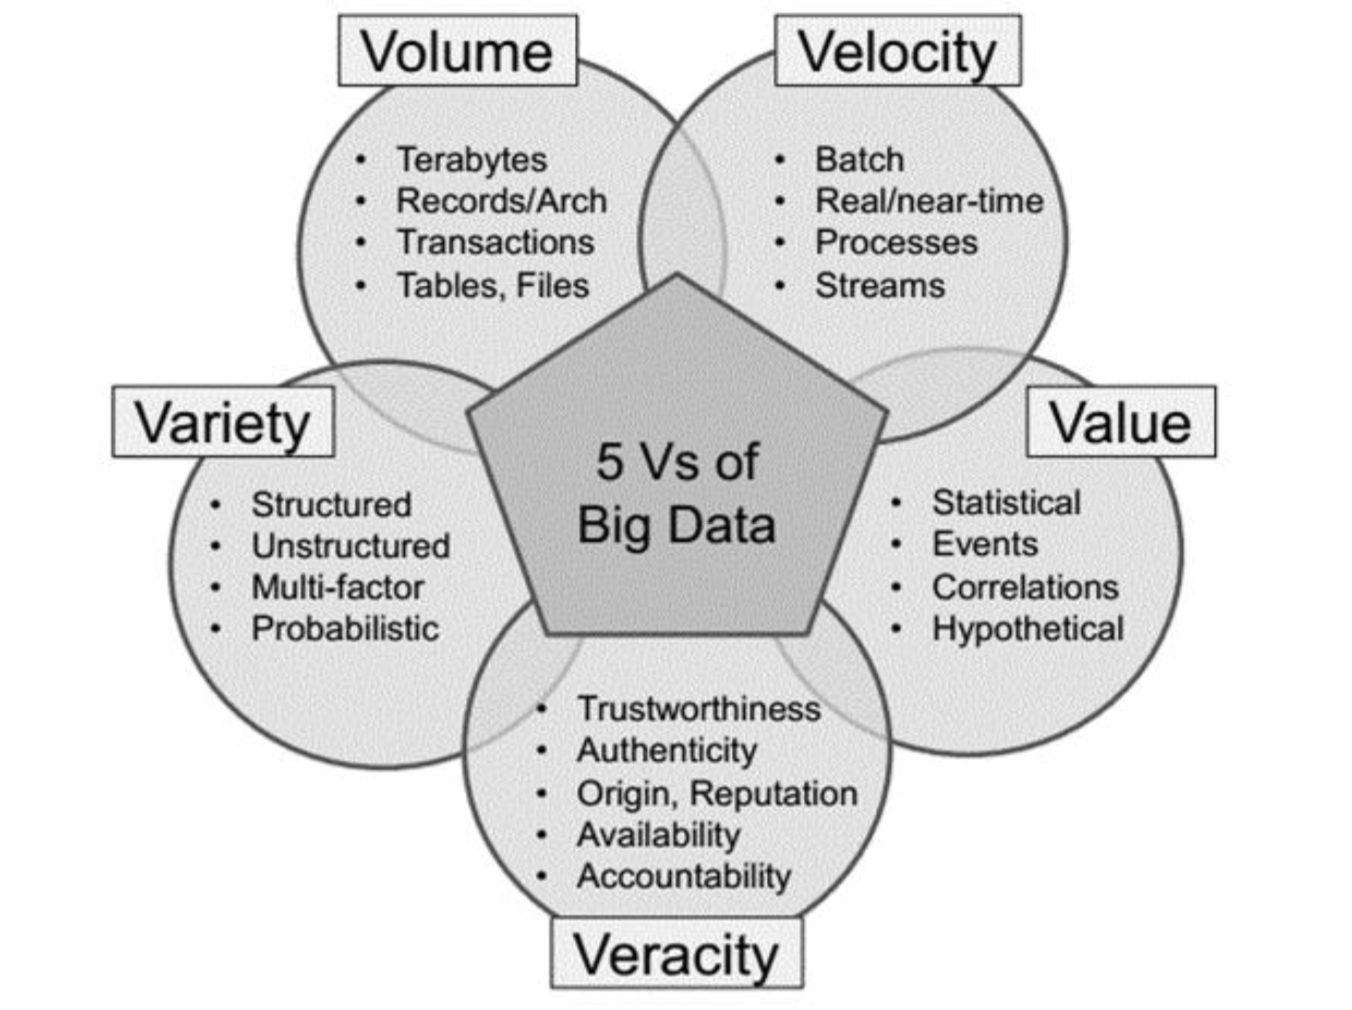
\includegraphics[width=0.8\textwidth]{{img/big-data-parameters}.png}\par}
  \caption{The \emph{5V's} of \acl{BDA}. Reprinted from \textcite[p.~81]{rajasekar2015survey}}
  \label{fig-5vs}
\end{figure}

\subsection{Challenges}
\label{sota-bda-challenges}

Although \ac{BDA} promises to serve as a major accelerator to companies' businesses as discussed beforehand, it is not trivial to implement and has some inherent difficulties. Based upon the challenges categorized and summarized by \textcite[p.~406\psq]{katal2013bd}, a wrap-up of commonly recognized challenges for the implementation of \ac{BDA} projects in the industry is given as follows:

\paragraph{Privacy and Security}
Labelled by Katal et al. as the most important issue to be concerned with, privacy and security aspects may have an impact not only on the feasibility of a given analytics project, but also entail serious legal consequences. Depending on the customer base and the specific environment such as country or age group, major violations of these aspects might have a significant negative impact on the company's brand sympathy and trustworthiness as viewed by the public. The major problem identified is the possibility of analytics to generate insights about individuals they are not aware of or they do not want others to know. Basing business decisions, such as advertisement targeting or price adjustments on such insights draws attention to ethical questions\,--\,although technical implementation of a project might be feasible, an in-depth investigation of such concerns will be necessary before rolling it out. The specific privacy and security concerns, alongside relevant laws and regulations for this project work will be discussed thoroughly in \autoref{sota-pol-legal}.

\paragraph{Data Access and Sharing of Information}
The ability to analyze data is obviously highly dependent on the presence of underlying data, requiring sophisticated data acquisition processes. This data acquisition might be associated with substantial costs, e.g. when paying for external access to data sources. Especially insights that are highly desired by businesses, such as benchmarks with their competitors, can usually not be realistically performed as there is no opportunity to acquire their competitors' internal data. Another obstacle in the data acquisition process is to gain the general consent to be allowed to analyze a data set; the sharing of information by data providers subsequently usable to harvest them becomes desirable. However, such data sets might not necessarily be very recent or even accurate. The insight that data access and quality play a key part for the competitive advantage in a modern business world follows trivially.

\paragraph{Storage and Processing Issues}
Due to the high volume and variety of data involved in modern \ac{BDA} projects (cmp. \autoref{sota-bda}), there may be issues with both its storage respectively processing. Although cloud computing offers virtually unlimited storage for end users, it is important to view both of these aspects in conjunction, leading to the conclusion that the highly distributed storage in various data centers, locations etc. usually leads to new problems associated with the processing of the data. The desire for a system offering solutions for both of these aspects, leading to a successful and powerful analytics platform appears to be large.

\paragraph{Analytical Challenges}
The major analytical challenges companies are confronted with when dealing with Big Data are associated with the aspects of volume and variety as well. The business somehow has to decide which data qualifies to be stored and analyzed, but especially how it should be set into perspective later on. Due to the desire to generate new hypotheses based on large data volumes, it is usually not clear beforehand which data points have to be regarded in order to create the most value for the organization. Furthermore, the variety of data usually requires large and expensive harmonization efforts to make data comparable or to be able to analyze it in an automated way. 

\paragraph{Skill Requirements}
Another important aspect of the implementation and feasibility of Big Data projects is the ability to execute well, thus creating actual value and acquiring reliable insights. This requires a well-trained workforce with sophisticated skills and expertise not only in the technical process of development and application, but possibly even more so in the part of harvesting results, thus requiring interpretative, analytical and research capabilities. Finally, even creative skills are desired, considering e.g. data visualization or exploration efforts.

\paragraph{Technical Challenges}
The following four major categories of technical challenges have been identified to need serious consideration when preparing and performing \ac{BDA} projects:

\begin{enumerate}
    \item \emph{Fault Tolerance} describes the ability of a system to be tolerant to defects or errors of its underlying components. In that sense, a analytics platform has to strive for a high level of fault tolerance, as perfect fault tolerance is generally not achievable. Fault tolerance is necessary to generate reliable and predictable results in the analysis process, without corrupting either the state of the system or its final results.
    \item With the enormous, ever-growing data sets to process, \emph{scalability} of the analytics platform is another major concern. Compute clusters have to adopt to varying degrees of use in order to maintain a sufficient performance level, while as storage clusters should be able to occupy the increasing data sets dumped into it. The usual procedure to achieve scalability is to join multiple smaller computing or storage nodes into a large cluster, together with some kind of cluster management that dispatches requests and orchestrates the underlying tasks. Such clusters are inherently hard to operate and especially data analysis algorithms that scale well while maintaining their descriptiveness and conciseness are hard to write.
    \item The \emph{quality of data} poses as a constraint for its derived insights. Although more data points will usually provide better insights in the case of decision making and predictive analysis, quantity generally does not compensate quality. As the time to process data is directly correlated to the size of the underlying data set, one should strive to analyze only the minimal data set necessary for the given problem.
    \item Finally, the \emph{heterogeniety of data} is becoming increasingly important with Big Data, preventing the usage of traditional systems that rely on data harmonization and fixed schemes. Coming up with a way to deal with such heterogeneous data is another one of the major obstacles of \ac{BDA}.
\end{enumerate}

\subsection{Exemplary Case Studies}
\label{sota-bda-use-cases}

to give a brief overview of how the concept of \ac{BDA} is employed in business, some exemplary case studies found in literature are summarized in this subsection.

\textcite{he2013social} describe the very prominent use case of social media analysis. The virtually unlimited data source of social media websites poses as the prime example of how mainly unstructured data may be aggregated in order to derive insights from it. In this case study, a competitive analysis of the three major American Pizza chains is performed, harvesting the \ac{BIA} 2.0 technique of text mining. This case study is particularly interesting as almost every company will need to address its customers in the public. Moreover, with social media the data source is not only nearly unlimited and updated in real-time but also publicly available, easing the cumbersome task of data acquisition. The real-time property of social media data allows businesses to react to sentiment changes of their customer base, e.g. following a new product announcement, in real-time.

Furthermore, a case study regarding the prediction of near-term trends is described by \textcite[p.~64]{mcafeebig}. Specifically, the researchers therein aimed to model the future movements of housing prices in the urban centers of the United States; as a sophisticated model of the \emph{National Association of Realtors} existed to serve as a benchmark, this case study allows to draw real conclusions regarding the possibility of \ac{BDA} to simplify businesses' research capabilities. In this case, the publicly available search data allowed to state more precise assumptions about future price movements than the results of the \enquote{professional} benchmark relying on extensive historical data and a quite complex model.



\section{Hadoop}
\label{sota-hadoop}
The \emph{Apache Hadoop Project} is a collection of tools that serves as a widespread platform for \ac{BDA} use cases nowadays. Contrary to common belief, Hadoop itself aims not to replace traditional \ac{OLTP} and \ac{OLAP} systems but rather complement them by offering a common platform for \ac{BDA} use cases that rely on such a massive data scale such old systems are not capable of processing anymore. Therefore, \autoref{sota-hadoop-components} will provide a brief overview of the foundational components among a short outline of the history of Hadoop. Moreover, an overview over the Hadoop ecosystem and its most prominent applications is given in \autoref{sota-hadoop-ecosystem}. Subsequently, these insights will be set into context in \autoref{hadoop-assessment}, creating a value assessment of Hadoop in the scope of \ac{BDA} and \ac{BIA}.

\subsection{Core Components}
\label{hadoop-components}
\label{sota-hadoop-components}

Hadoop is mainly made up of two flexible and scalable core layers: \emph{storage} and \emph{processing}. This subsection iterates over these layers by showing the inspiration, supporting principles and derived advantages of their application.

\subsubsection{File System}
The storage layer is formed by the so-called \acf{HDFS}, which serves as a distributed file system that may run on clusters of arbitrary sizes and is heavily inspired by Google's \ac{BFS} paper by \textcite{ghemawat2003gfs}.

The first advancement of \ac{BFS} in comparison to earlier distributed file systems is to expect failure of cluster nodes to be the norm rather than an exception: This becomes especially important when running the cluster on top of so-called \enquote{commodity hardware} \autocite[p.~1]{ghemawat2003gfs}, that means comparatively cheap consumer hardware rather than expensive enterprise server equipment. This drives down the costs of the cluster, as no premiums for high-availability features and expensive support contracts have to be paid, however to the expense of reduced availability of single nodes \autocite[p.~1]{ghemawat2003gfs}. As the file system is expecting such failure, data blocks are replicated across multiple nodes, leading to an availability guarantee approaching 100 per cent as the cluster grows \autocite[p.~2]{ghemawat2003gfs}. Secondly, rather than storing hundreds of thousands of small files as with traditional file systems, \ac{BFS} is designed to work with far fewer, yet larger files, often with sizes ranging from gigabytes to terabytes \autocite[p.~2]{ghemawat2003gfs}. Furthermore, rather than using random access, the file pointer is usually moved only linearly, resulting in an append-only mode for writing data as well as batch processing for reading data \autocite[p.~2]{ghemawat2003gfs}. Finally, the file system is custom-tailored for the applications running on top of it, rather than serving as general purpose implementation \autocite[p.~2]{ghemawat2003gfs}.

Adapting these principles \ac{HDFS} was created as a seamlessly integrated, integral part of the Hadoop system. To implement the storage system, 
Hadoop defines two services that form the infrastructure for \ac{HDFS} which runs on the nodes. Data in the file system is distributed among multiple \emph{datanodes} which store blocks of files. In the cluster there is exactly on \emph{namenode} service node which keeps track of where the blocks of each file are located and how they can be retrieved. Utilizing the principles of \emph{sharding} and \emph{replication} the files stored in \ac{HDFS} are split into blocks and saved on multiple \emph{datanodes}. There can be a \emph{secondary namenode} which  mirrors the primary and can be act as a fail-over instance. Figure \autoref{fig:hdfs_read} visualized this architecture and illustrates how a client reads data from \ac{HDFS} by first contacting the \emph{namenode}, requesting the block locations and subsequently contacting the \emph{datanodes} directly to read the actual data.

\begin{figure}[htb]
     {\centering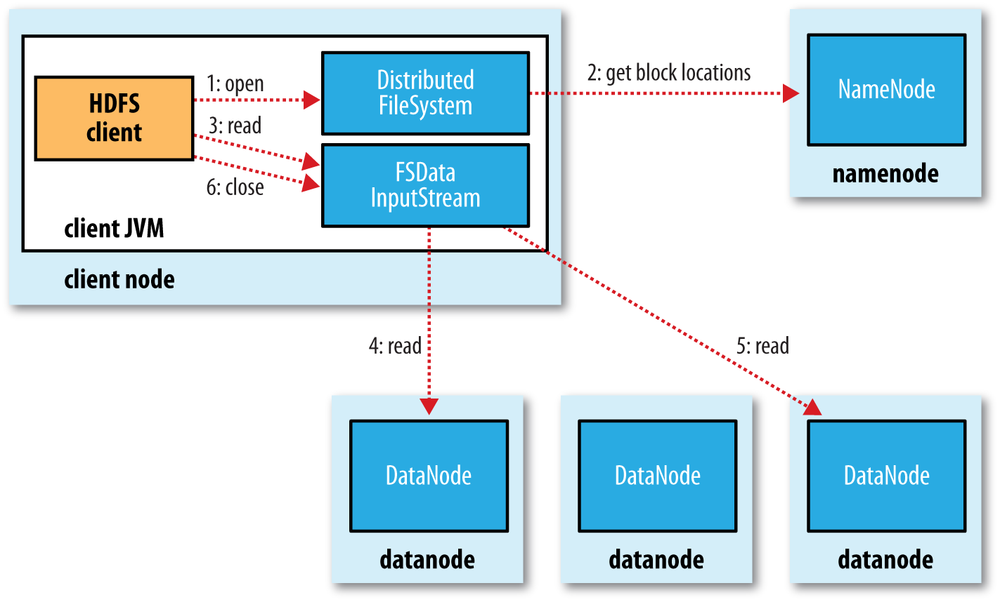
\includegraphics[width=0.75\textwidth]{img/hddg_0302.png}\par}
	\caption{Schematic Overview of a \ac{HDFS} request and its associated nodes in a Hadoop cluster. Reprinted from \textcite[][Chap.~3]{white2015hadoop}.}
	\label{fig:hdfs_read}
\end{figure}

\subsubsection{Processing Framework}

Building upon this storage layer is the processing layer, which serves as the interaction point for developers, data scientists and other users of the system. The processing layer of Hadoop did undergo some major changes before the release of its second version \autocite[p.~5]{vavilapalli2013apache}; for the sake of completeness and contextual understanding both versions are subsequently outlined.

The first version of Hadoop was heavily influenced by a second important Google paper, \textcite{dean2004mapreduce}, introducing the batch processing algorithm MapReduce \autocite[p.~82]{rajasekar2015survey}. Each MapReduce job can be designated as $J: (M, R)$ with the map function $M: (k_1, v_1) \rightarrow list(k_2, v_2)$ and the reduce funcion $R: (k_2, list(v_2)) \rightarrow list(v_2)$ \autocite[p.~6]{dean2004mapreduce}. The job runner now calls $M$ for each data chunk in parallel on possibly many different nodes, resulting in the intermediate result. In a second step, upon completion of all map functions, the $v_2$ values are joined as a list by the value of their respective $k_2$, and subsequently passed to $R$, again running parallelized on multiple cluster nodes \autocite[p.~6]{dean2004mapreduce}. As outlined in the paper, a variety of data processing operations can be expressed very briefly and without concerning the programmer with the difficulties of writing a distributed, well-scaling algorithm \autocite[p.~6]{dean2004mapreduce}. The simplicity of the MapReduce pattern thus lead to a widespread adoption for various use cases across many industries as their primary batch processing framework running on-top of Hadoop \autocite[p.~82]{rajasekar2015survey}.

Although the MapReduce approach is largely suitable for its intended use case of web crawling, among others, it is however not generally the best programming model to solve arbitrary data analysis and processing tasks.
As becomes obvious by the function definitions before, MapReduce jobs are limited to the analysis of isolated \enquote{data snippets}; finding or even investigating the relations and interdependence of larger data agglomeration quickly becomes a sophisticated, cumbersome task.

Due to the tight coupling of Hadoop 1's storage and processing layer, the design of Hadoop was inherently limiting its merit and the extent of applicable use cases. Thus, \ac{YARN} was developed as an abstraction layer between the traditional \ac{HDFS} storage layer and applications performing the data processing itself, creating a more flexible, powerful and even performant platform rendering the unintended use of MapReduce obsolete and limiting the scope of the MapReduce programming model to merely be one of the possible processing frameworks running on top of \ac{YARN} \autocite[p.~6]{vavilapalli2013apache}.

In 2013, \ac{YARN} was incorporated into the second major release of Hadoop \autocite{hadoopreleasenotes}, completing the transformation of Hadoop from being a limited, MapReduce-focused data processing platform to become a single, extensively applicable \ac{BDA} platform. Due to this change, creating processing frameworks as well as applications on top of Hadoop became easier to implement and maintain; furthermore, it stopped the abuse of MapReduce in earlier implementations, where massive data duplication and transient storage was required to mitigate the shortcomings of MapReduce for the holistic inspection and analysis of stored data.

To implement the \ac{YARN} infrastructure, Hadoop introduces two services that can be deployed on the cluster nodes.
The \emph{ResourceManager} accepts application requests from clients and handles the management of computation resources in the cluster.
It can allocate new \emph{containers} on the cluster nodes, which encapsulate resources and execte the application .
There is only one \emph{ResourceManager} in the cluster.
Each node that performs data processing is running the \emph{NodeManager} service which receives jobs and executes them inside a \emph{container}.
If more resources are needed dynamically, the application running on the \emph{NodeManager} can request more resources from the \emph{ResourceManager}.
Figure \ref{fig:yarn} illustrates this behavior in a typical application execution.

\begin{figure}[htb]
     {\centering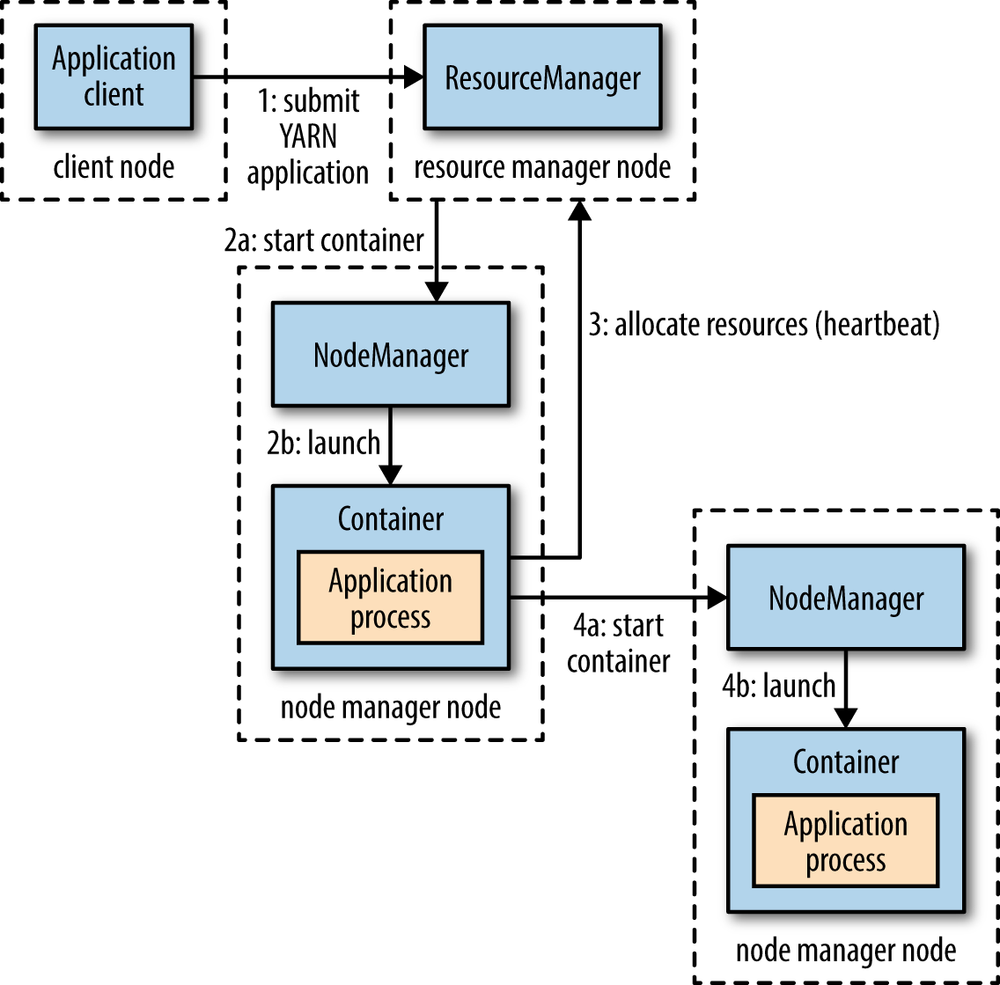
\includegraphics[width=0.75\textwidth]{img/hddg_0402.png}\par}
	\caption{Schematic Overview of the subprocesses and their associated executors of a \ac{YARN} task. Reprinted from \textcite[][Chap.~4]{white2015hadoop}.}
	\label{fig:yarn}
\end{figure}

\subsection{Map Reduce Shortcomings}
\label{sec:fund:mapred_shortcomings}

The growing number of Hadoop based frameworks (as visible in \ref{hadoop-ecosystem}) and applications demonstrates, that using simple MapReduce based algorithms is not sufficient and flexible enough, given the amount and diversity of data gathered today.

The most common issues faced by Hadoop, are caused by the limitations of the two stage MapReduce algorithm \autocite[][]{6903263}. 

MapReduce was originally developed to batch process data and is
therefore not the optimal solution to perform different kinds of
workloads that cannot be easily expressed in this
way \autocite{computers3040117}.
To approach this problem tools have been crated that follow different methods, while still utilizing \ac{HDFS} and \ac{YARN}.

In order to find an optimal solution for approaching different kinds of problems, various processing tasks usually found to be processed on Hadoop clusters may be grouped in the following ways \autocite{computers3040117}:

\paragraph{Real-time Processing}
Real-time Processing aims to reduce the response time of MapReduce jobs to allow them to be used for real-time queries and analysis. As \textcite{computers3040117} stated, one of the reasons for slow MapReduce response times is the \ac{HDFS}, which is \enquote{designed for high throughput data I/O rather than high performance I/O}.
Therefore, while MapReduce may be a powerful tool to perform batch processing, its overhead is too high to be used in any kind of real-time setting \autocite{computers3040117}.

\paragraph{Stream Processing}
While real-time processing is something MapReduce can, albeit poorly, still do, its set of features does not allow for native stream processing. MapReduce is build to run on batches of data with a very fixed cycle of:
\begin{enumerate}
    \item Gathering all the input data
    \item Running MapReduce to compute the output
    \item Returning all the output data
\end{enumerate}
This limits Hadoop with Map Reduce to use cases where all the data is known before.
However Tools such as \emph{Apache Kafka} and \emph{Apache Samza} can run on Hadoop to enable stream processing use cases with.

\paragraph{Graph Processing}
Graph processing is becoming increasingly relevant for
applications in industry and academia. 
As a general purpose computation framework Hadoop 
can be used together with MapReduce to run calculations 
on large graph datasets, 
but it generally is not optimized for such workloads \autocite[][]{Capota:2015:GBD:2764947.2764954}. 
Tools optimized for graph-like data structures can utilize algorithms that are especially optimized for graphs, instead of the general purpose MapReduce.
Examples for such tools are \emph{Apache GraphX} and \emph{Apache Giraph}.

\subsection{Hadoop Ecosystem}
\label{hadoop-ecosystem}
\label{sota-hadoop-ecosystem}

One of the major advantages of Hadoop is its rich ecosystem. Hadoop clusters can be extended to serve a very wide range of purposes that are not covered by the traditional combination of \ac{HDFS} and MapReduce. As Benjelloun et~al. establishes, components in the Hadoop ecosystem may be grouped into the following categories \autocite{7105553}:

\paragraph{Data Integration}
Data integration tools such as \emph{Apache Flume} or \emph{Apache Sqoop} manage the transfer and import of large amounts of data from relational databases \autocite{apache2018sqoop}, event streams and other data sources \autocite{apache2017flume} into a Hadoop cluster.

\paragraph{Resource and Cluster Management}
Management tools like \emph{Apache Ambari} and \emph{Apache ZooKeeper} simplify the deployment, monitoring and general management of Hadoop clusters. Together with \ac{YARN} for low level resource management, and \emph{Apache Oozie} for workflow management, these tools partially define how Hadoop is used and are important to keep a cluster efficient.

\paragraph{Metadata Services}
This smaller category contains tools like \emph{Apache HCatalog}, that offer a common interface between other Hadoop data processing tools \autocite{bmc2017hcatalog}. Since most tools have a specific format that is used to read and write data, \emph{HCatalog} simplifies their integration by eliminating the need for manual data conversion \autocite{bmc2017hcatalog}.

\paragraph{Data Analytics}
Data analytics tools like \emph{R} work well together with Hadoop to give data scientists 
a familiar interface for analysis of the data aggregated in Hadoop. Additionally, machine learning frameworks like \emph{Apache Mahout} can use Hadoop to perform computationally expensive mathematical calculations on a cluster to gain deeper insights into the gathered data. For more simple operations, \emph{Apache Hive} may be used.

\paragraph{Search and Querying}
Search and indexing tools simplify and speed up the process of querying data stored on the \ac{HDFS}. Different tools are often optimized for a specific set of data structures and use cases. Commonly used in this context are \emph{Elasticsearch-Hadoop} or \emph{Sphinx} for full-text search, \emph{Facebook Unicorn} for graph search and \emph{Apache Hive} for \ac{SQL} like queries.

\paragraph{Data Visualization}
While data analytics tools can be used for detailed analysis, their usage is preceded by data visualization tools such as \emph{Centrifuge}, offering a high level overview over the available data. These tools can be used to discover insightful connections and visualize sections of the data.

\paragraph{Data Processing}
Since MapReduce is not the optimal choice for every type of workload as discussed above, data processing frameworks like \emph{Apache Pig} and \emph{Apache Spark} that offer a richer set of features can be used for more complicated data processing and transformation workloads. Instead of using general purpose tools, more specialized processing engines such as \emph{Apache GraphX} or \emph{Apache Giraph} can significantly improve the processing speed.

\paragraph{}
This wraps up the most common and interesting categories of \ac{BDA} tools compatible with Hadoop. It is important to note that many tools do not fit perfectly into these categories and can often be used for multiple purposes. \emph{Jonas Balsfulland}'s report investigates the characteristics and usage of these tools in more detail.

\subsection{Value Assessment}
\label{sota-hadoop-assessment}
\label{hadoop-assessment}

This subsection focuses on setting the previously acquired knowledge relating \ac{BIA} and \ac{BDA} into the context of Hadoop, especially with regards to the feasibility of Hadoop to support various kinds of workloads and cover a high percentage of desired use cases. Therefore, the general problems and challenges of \ac{BDA} (cmp. \autoref{sota-bda-challenges}) are related to Hadoop's specific properties and components in the following.

\paragraph{Privacy and Security}
Hadoop has been designed as an append-only storage environment. This entails some serious consequences in the context of privacy, as the business desire is that individual data items should not be deleted at any time to allow for further analysis and transparency. In the light of recent regulations, especially relating to the \ac{GDPR} in the \ac{EU}, this is not legally compliant. Because of its major importance, this topic will be covered in-depth in \autoref{sota-pol-legal}. The ethical questions concerned with whether to implement a certain project or not are not limited to its analytics platform and project specific and will therefore need individual judgement. Looking at security, it can be said that Hadoop currently does not enforce a high level of security per se, as neither storage nor transport level encryption are supported so far on a software level \autocite[p.~82]{rajasekar2015survey}, due to complexity and performance issues. However, it is possible to implement storage level encryption on a hardware level. The lack of transport level encryption however has to be noted and leads to the consequence that Hadoop clusters should be operated in a separated, at least virtually distinct network protected from intruders on a higher level. On a logical level, data can be protected in \ac{HDFS} with \acp{ACL}, allowing for a granular access allocation of available data to its users \autocite{hdfspermissions}.

\paragraph{Data Access and Sharing of Information}
The ability of an organization to source external data is obviously out of scope of the analytics platform in use. However, it becomes important that Hadoop may store any data in arbitrary form, making the integration of new data sets as easy as uploading files. On an internal level, Hadoop promotes the sharing of information by offering a central data storage that should be available to any employee concerned with business development, data analytics and even more areas. Through regulatory requirements, unlimited access will be rare, however users should be made aware of the data available in order to request access if needed and legally compliant. The \emph{DataOps Manifesto} emphasizes the need of organizations to focus on viewing analytics as a processual, value-adding functional area that should always be reproducible in order to share not only the resulting knowledge but also the means of how to achieve it \autocite[§11, §14, §17]{dataopsmanifesto}. Hadoop fits nicely into this concept, as it promotes the reuse of data and eliminates organizational boundaries that would otherwise serve as a source of operational friction.

\paragraph{Storage and Processing Issues}
This challenge area has arguably been the focus in the design and architecture of Hadoop. Therefore, Hadoop solves the capacity limits of traditional environments by offering capabilities to linearly scale the cluster's size by simply adding new nodes of commodity hardware. This positively impacts both the storage as well as the processing power. Through its sophisticated processing frameworks, including applications running on top of Hadoop for specialized use cases, a very extensive ecosystem exists to solve a wide varying array of business cases. A caveat worth noting is the maturity of this ecosystem; although some frameworks are widely used in the enterprise world and are undergoing active development, they do not have professional organization backing e.g. \acp{SLA} or other contracts that guarantee the implementation of new functionality as well as bug and security patches.

\paragraph{Analytical Challenges}
The analytical challenges can be mitigated by Hadoop only in a limited manner, as it mainly is a problem area to be addressed by business decisions (e.g. which data to upload or process). However, by offering data visualization and exploration capabilities through applications in its ecosystem as outlined in \autoref{sota-hadoop-ecosystem}, this task can be supported by Hadoop to some extent as well.

\paragraph{Skill Requirements}
Hadoop offers extensive documentation guiding users through the use of a cluster. Yet, the operation and setup of Hadoop clusters is a complex task. The automation of this is one the goals of the authors project work, leading up to quicker roll-outs of new clusters and/or their reproducible set up. Moreover, a substantive set of professional services firms exist on the market that may support an organization to execute well with their analytics efforts \autocite{hadoopconsulting}. Undoubtedly however, especially academic programs will need to catch up with the recent and future developments in order to satisfy the growing market's desire for talent supporting these efforts.

\paragraph{Technical Challenges}
The four categories of technical challenges are wrapped up in \autoref{fig-hadoop-technical-challenges}. It should be noted that Hadoop addresses most of the technical challenges in a fair way, especially offering great scalability and fault tolerance. The more \enquote{soft} characteristics of quality and heterogeniety mainly rely on the best effort of the organization as well as its employees to collect the right data and use the appropriate tools offered by the Hadoop ecosystem to solve their problems.

\begin{table}[hbt]
    \centering
    \resizebox{\textwidth}{!}{%
	\begin{tabular}{p{3cm} p{7cm} p{7cm}}
	  Characteristic & Advantages & Disadvantages \\
	  \hline
	  Scalability & Supports thousands of nodes for data storage and processing. Scales almost linearly with the cluster size. High block size enables the efficient, distibuted storage of vast amounts of data & Only suitable for \enquote{real} Big Data applications, not for general purpose data storage (e.g. small files)\\
	  Fault Tolerance & Resilient to the failure of nodes, both in software and hardware (excluding the name node) & The name node serves as a single point of failure, however a secondary name node can be configured to mitigate the data loss\\
	  Quality of Data & The original data is persistently stored, and through its append-only approach, Hadoop clusters may reconstruct the data available at any point in time in order to retrospectively perform analyses & High effort for the analytics engineers to harmonize the unstructured data on-read. Mitigated in part by frameworks supporting these efforts. However, the accuracy and precision of stored data cannot be guaranteed and relies on the using organizations' policies and e.g. process steps before data is uploaded to the cluster\\
	  Heterogeniety of data & Large ecosystem of applications based on \ac{HDFS} and \ac{YARN}, covering nearly all common use cases & Parts of the ecosystem are non-mature and still under development
	\end{tabular}}
	\caption{Technical Advantages and Disadvantages of the Apache Hadoop Platform. Partly adapted from \textcite[p.~82]{rajasekar2015survey}}
	\label{fig-hadoop-technical-challenges}
\end{table}

\paragraph{Conclusion}
The points above discussed in-depth both the advantages and disadvantages of Hadoop in order to assess the aptitude of Hadoop as an analytics platform in the context of \ac{BDA}. In general, it can be said that Hadoop currently offers the most extensive and powerful solution for organizations that seek to satisfy their desire for an integrated, powerful, scalable and fault-tolerant analytics platform. The biggest problems with Hadoop itself exist in the area of \textbf{Privacy and Security}, where the current approach of an append-only environment clashes with individuals' interests for privacy, anonymity and non-interference with their personal life. Although being very mature in a technical sense, these governance and compliance problems will be of major interest in the future when organizations decide whether and how to realize their analytics efforts.

\subsection{Hadoop at the DHBW}

Being a academic institution with direct contact to 
business partners in the technology industry the \ac{DHBW} has an interest to cover recent developments in a variety of fields in their lectures and studies.
Since Big Data is a currently emerging topic,
the \ac{DHBW} Stuttgart currently offers multiple that lectures incorporate this topic.
In the course of study in applied computer science within the faculty of engineering there are three courses that are integrated into the studies for the Bachelor of Science.
The lecture \emph{Databases II} deals with concrete database implementations and current developments in databases as well as with Data Warehouse architectures and implementations \autocite[][]{DHBW2017aidbii}.
The optional lecture \emph{Cloud-Applications, DevOps and Big Data} also covers the ecosystem for Big Data in cloud environments \autocite[][]{DHBW2017aiwf}.
Furthermore there is another optional course on \emph{Data Science} introduced in 2018 which covers the basics in algorithms, metrics and tools needed to perform data analysis and machine learning.
These courses already include Hadoop in their lecture content to varying degrees.

Starting with the winter semester 2018 the \ac{DHBW} Mannheim will offer a new course of study in \emph{Data Science} for the Bachelor of Science at the faculty of business.
It will focus on a datacentric view and addresses current developments in businesses that make Big data the foundation for decision making and income generation.
\autocite[][]{DHBW2018mannheimdatascience}

Each of the mentioned courses holds the possibility to come in contact with Hadoop in some way and explore current topics in its development, functionality and usability - be it from a business point of view, from a technical system view or with a concrete example case that can be explored hands-on by the students.
By having a possibility to use Hadoop within the \ac{DHBW} students and teachers alike can profit in the way Hadoop can be taught.

\section{Political and Legal Framework}
\label{sec:fund:legal}
\label{sota-pol-legal}

When a \ac{BDA} system is actively used, it handles data in diverse forms from many sources. Depending on the kind of data, there are different legal restriction to the conditions of collection, storage and processing thereof. The major restrictive laws that are applicable for the \ac{DHBW} are the European \ac{GDPR}, the German \ac{BDSG}\,--\,the Federal Data Protection Act\,--\,and the \ac{HSchulDSV} Baden-Würtemberg\,--\,the data protection regulations for institutions of higher education.

The \emph{\ac{HSchulDSV} in Baden-Würtemberg} regulates which personal data the \ac{DHBW} may collect from students and how this data may be used. It permits the usage of personal data for \enquote{organizational or other purposes} and allows the creation of anonymized reports with it \autocite[§1, §11, §12]{bw2012hcchuldsv}. Personal information about students must be deleted 40 years the the student was exmatriculated \autocite[§1, §11, §12]{bw2012hcchuldsv}.

The \emph{German \ac{BDSG}} regulates the general principles of data protection in Germany and restricts the collection, usage and storage of personal data. In general, no more data than necessary may be collected and the processing of data requires the explicit user's consent \autocite[§1ff.]{bmjv2009bdsg}. The user may also demand the deletion of their data at any time \autocite[§12ff.]{bmjv2009bdsg}.

The \emph{European \ac{GDPR}} is largely based on the German regulation and introduces more control for users about their personal data \autocite{eu2016gdpr}. The \ac{GDPR} Portal \autocite{trunomi2018gdpr} summarizes the key changes introduced by the new regulations:
\begin{itemize}
    \item \emph{Penalties} may be imposed for organizations that breach the \ac{GDPR}.
    \item \emph{Consent} from users must be requested to collection, storage and usage of personal data. The consent may be revoked.
    \item \emph{Breach Notifications} are mandatory to inform users if data was exposed.
    \item \emph{Right to Access} for every user to their own personal data.
    \item \emph{Data Portability}, i.e. the requested data should be available to the user in a common format.
    \item \emph{Right to be Forgotten}, i.e. the right to have personal data deleted permanently upon request.
    \item \emph{Privacy by Design} for new data processing systems.
\end{itemize}

Especially the \emph{right to be forgotten} is problematic in \ac{BDA} systems
since data can be stored in an unstructured, immutable way. This restricts the possibility to keep track of which data entries are actually stored in the system. Deletion is therefore practically impossibly. To circumvent this restriction, extra caution is necessary to decide which data should be used on the platform. 

The listed laws focus on personal data, but might also be applicable to anonymized data that is derived from personal data. Table \ref{fig-legal-data-kinds} describes which restrictions and/or regulations apply to which type of data from which source. An example for the kind of data is given. Note that open source personal data sets are fundamentally not available since public unrestricted distribution of personal data contradicts with the \ac{GDPR} and no public initiative to collect such data is known to the author.


%\newcommand{\myoldarraystretch}{\arraystretch} % very bad idea
%\renewcommand{\arraystretch}{1} % very bad idea

\begin{table}[hbt]
\resizebox{\textwidth}{!}{%
	\begin{tabular}{l|lll}
	  Kind of Data & Internal & Open Source & Closed Source \\[0.5em]
	  \hline\\[-0.5em]
	  Personal & \acs{GDPR} \& \acs{HSchulDSV} & N/A & \acs{GDPR} \& license \\
	  & e.g. student data & N/A & e.g. advertising contacts\\[1em]
	  Anonymized & possibly \acs{GDPR} \& \acs{HSchulDSV} & possibly \acs{GDPR} & possibly \acs{GDPR} \& license\\
	  & e.g. lecture statistics & e.g. social media graphs & e.g. advertising statistics\\[1em]
	  Non-Personal & unrestricted & unrestricted & restricted by license \\
	  & e.g. server monitoring & e.g. weather data & e.g. bought datasets \\
	\end{tabular}%
	}
	\caption{Different combinations of data sources and types with their respectively applicable laws, regulations and licenses in the context of the \acs{DHBW}}
	\label{fig-legal-data-kinds}
\end{table}

% \renewcommand{\arraystretch}{\myoldarraystretch}% very bad idea

When the Hadoop cluster is used at the \ac{DHBW}, it might by accessed by administrative staff, lecturers and students. However, as Hadoop had not been designed with advanced user access and the ability to delete single records in mind, care must be taken regarding the question which types of data from which data sources should be stored on the cluster. The least restrictive solution is to use a public, open source, non-personal data set, such as academic research data, while avoiding the storage of personal student data on the cluster.
% !TEX root = ../master.tex
\chapter{Design}
\label{chap:design}

\section{Analysis of Cluster Environment}

The Hadoop cluster will be installed on the cluster computer at the \ac{DHBW} Mannheim.
This cluster utilizes \emph{OpenStack} \urlinline{https://www.openstack.org/} to provide resources to its users. 
OpenStack is an open source project to manage cloud computing architectures.
It enables the compositions of compute elements (virtual machines), network elements (sub-nets and routers), 
and storage elements (virtual disks) to form a virtual computing environment.
The OpenStack management web interface can be accesses at \urlinline{https://controller.c4.dhbw-mannheim.de/} from within the \ac{DHBW} network. 
The \emph{Cloud Computing Competence Center} at the \ac{DHBW} Mannheim  manages the cluster computer.

The OpenStack environment is shared between multiple user groups, 
which each is given a certain amount of resources. 
For this project the student group is given a limited amount of resources.
Only 20 virtual \ac{CPU} cores, 50 \ac{GB} \ac{RAM} and 1 \ac{TB} of storage are dedicated to the project.
This resources can be used to allocate instances of \acp{VM} in pre-defined units and assign virtual disks to them.
The \acp{VM} can be connected to the network of the \ac{DHBW} and can be interconnected using internal, virtual networks.
Firewall restrictions can be set through group policies, which can be assigned to the \acp{VM}. 
When creating a new \ac{VM} most of these settings must be supplied. 
Furthermore the operating system flavour can be chosen and a \ac{SSH} login key can be provided.
Among others \emph{Ubuntu 16.04 LTS} \urlinline{https://www.ubuntu.com/server} can be used which is compatible with Hadoop in general.

The Hadoop cluster be deployed on multiple interconnected \acp{VM} in the OpenStack environment that can be accessed from the university network.

The connection to the \ac{DHBW} network gives some restrictions: \acp{VM} can only be accessed from the university network and not from the Internet.
From a security point of view this decreases potential attac vectors.
However for development access it is restricting, 
since the developer needs to be on premise. 


\section{Analysis of Requirements}

There are three main user groups that can be determined for the Hadoop cluster:

\begin{itemize}
    \item \textbf{IT Staff} -- The technical staff at the \ac{DHBW} can perform maintenance on the Hadoop cluster and possibly a re-setup of it.
    Also they might use it for research projects.
    \item \textbf{Lecturers} -- Lecturers might most likely use the cluster for the purpose of teaching classes about \ac{BDA} and give hands on experiences for the students. They might prepare the educational material and data sets on the cluster and exemplary demonstrate its usage.
    \item \textbf{Students} -- Students at the \ac{DHBW} might use the cluster within the context of courses or research project to perform data analysis. Within lectures they might be instructed by the teacher, in research project they can use the cluster on their own.
\end{itemize}

In his paper, \emph{Philipp Winter} discusses more possible use cases for the cluster. It focuses on the educational usability in lectures.
(TODO write about this paper, what is it really)
Main users are lecturers and students to perform analytics of various data on the cluster.

Sicklinger et al. also did a requirements analysis for an Hadoop cluster at the \ac{DHBW}. 
\begin{itemize}
    \item The cluster utilizes the OpenStack Environment in Mannheim.
    \item There should be only a low cost, at best no cost, associated with deploying and running the cluster.
    \item It should be possible for students and lecturers to deploy the cluster.
    \item The cluster should provide the ability to be used to learn about the Hadoop deployment and learn about data analysis.
    \item The it should support recent tools to be used alongside with Hadoop.
    \item The cluster should scale to the needs of the users.
\end{itemize}
\autocite[][p. 40ff]{wi2018managementsystems}


All of the listed requirements imply that the cluster needs to be deployable without extended or expert knowledge about Hadoop itself.
Automated deployment is therefore favourable to make the procedure reproducible. 
Still it can be required for the person performing the installation to have general knowledge about system administration on Linux based machines.


\section{Research on Possibilities}

After the requirements are settled,
the possibilities of how Hadoop can be installed 
on the given infrastructure will be researched. Therefore first a understanding how Hadoop clusters can be deployed and maintained more efficiently using \emph{Cluster Management Systems} is established.
Then possible ways to install Hadoop are evaluated experimentally and features and drawbacks of each approach are laid out.
This will lead to an decision on the method that should be used for the cluster at the \ac{DHBW}.

\subsubsection{Cluster Management Systems}
\label{sec:design:clustermanagement}
To deploy Hadoop on an cluster there are two general approaches. Either the Hadoop distribution package is installed and configured manually on each node or an management tool is used to perform automatic deployment and configuration. 
Since the manual installation process is error prone (as visible in section \ref{sec:design:manualinstall}) and needs some know-how,
it is  more easy for the user to utilize an management system for the cluster.

The management system can provide, install, manage and monitor software components on the cluster nodes.
Not only \ac{HDFS} and \ac{YARN} can be deployed,
but also additional tools can be integrated into the cluster this way.
Usually the management system also provides an graphical user interface to perform those tasks.

To provide the components the management system downloads them from a given binary distribution repository. The installation can be performed via remote access from the management server to the nodes. Monitoring gives valuable information to the cluster user, such as capacity an utilization of computational power and storage.

\subsubsection{Hadoop Distributions}
Some vendors choose to bundle a management system 
together with an specific version of Hadoop and additional Tools. They offer this bundle mostly as binary packages which are considered \emph{distributions} of Hadoop.
For system maintainers this holds the benefit that no compilation from source is necessary and the versions of the tools are adjusted to work with each other. 
Notable distributions are \emph{\acf{CDH}} and \emph{\acf{HDP}}. 

There are four ways to install Hadoop that are considered here:

\begin{itemize}
    \item A \emph{manual installation} of Hadoop 
        and every additional piece of software from the ecosystem
    \item \emph{\acf{CDH}} --  An open source software distribution by Cloudera including Hadoop
        and additional software from the ecosystem
        \urlinline{https://www.cloudera.com/products/open-source/apache-hadoop/key-cdh-components.html}
    \item \emph{Ambari} -- An open source project by Apache that provides
        the capability to manage Hadoop Clusters and the software components running on it.
        \urlinline{https://ambari.apache.org/}
    \item \emph{\acf{HDP}} -- Hortonswork's ready-to-install distribution of Hadoop 
        with Ambari and additional software
        \urlinline{https://de.hortonworks.com/products/data-platforms/hdp/}
    \item \emph{MapR} -- Commercial Hadoop distribution by MapR Data Technologies, Inc. A community edition is available. \urlinline{https://mapr.com/}
        
\end{itemize}

Since \ac{HDP} makes use of Ambari for installing the cluster and managing the installed software \autocite[][]{hortonworks2018ambari} while it simply provides a pre-packaged version of the components, 
it can be preferred over using Ambari directly which would create the need to compile it from source.

\emph{MapR} will not be discussed, since its free-of-charge community edition is only permitted to be used for \enquote{[internal] trial, evaluation, testing or similar non-production purposes} \autocite[][para.~1.5]{mapr2018EULA}. 
It therefore does not qualify to be used permanently at the \ac{DHBW} for educational purposes.

In the next sections the remaining three options, 
\emph{manual installation, \ac{CDH} and \ac{HDP}}
are tested and compared by performing a exemplary installation.
Each of the evaluations considers the complexity and susceptibility to error of the installation process.


\subsubsection{Evaluation Environment}
In the coming sections each of those three resulting possibilities will be looked at in more detail.
For each of the options an evaluation will be made on whether it is 
feasible to deploy an Hadoop installation with the methods that they provide.
Therefore a simple test installation in an OpenStack environment is made.
For this purpose the OpenStack environment \emph{BWCloud} \urlinline{https://www.bw-cloud.org/de/projekt}
is used, an environment that is available for students at the \ac{DHBW} 
and other universities in Baden-Württemberg for educational purposes. 
It is generally an equivalent software to the actual cluster environment, 
however it is accessible from the Internet, 
which makes it more comfortable to work with while performing the tests.

\subsection{Manual Installation of Hadoop}
\label{sec:design:manualinstall}

The first possibility to install Hadoop onto a number of hosts 
is to use the installation package provided by Apache them self \urlinline{https://hadoop.apache.org/releases.html}.
This represents the most basic procedure of installation.
Tom White \autocite[][Appendix A]{white2015hadoop} describes how Hadoop can be manually installed on the machines in an cluster. 
Manually here means without the help of automated installers for a single machine or the complete cluster. 
Every aspect of the installation and configuration must be done \enquote{by hand}.
White gives step by step instruction on the process.

Since no step in this step is predetermined or automated, this method does not really install an "Hadoop distribution" on the cluster, but rather only \ac{YARN}, \ac{HDFS} and MapReduce.
It does not provide a \emph{management system} for Hadoop.

\subsubsection{System Setup}
For the installation two \acs{VM} are used, utilizing two virtual \ac{CPU} cores and eight \ac{GB} \ac{RAM} and a 20 \ac{GB} storage drive. 
Ubuntu Serve 16.04.3 \ac{LTS} is used as the operating system. 
The machines are connected to the public Internet and to each other using two network interfaces each.

The two machines are going to be connected together in an master-slave setup
where the master runs the \ac{YARN} resource manager and the \ac{HDFS} name node as well as an \ac{HDFS} data node and an \ac{YARN} client node.
The slaves runs only an \ac{HDFS} data node and an \ac{YARN} client node.

First the system of the master is configured. Therefore the following steps are taken.

\begin{enumerate}
    \item The system is updated and OpenJDK 1.8 \urlinline{http://openjdk.java.net/}  is installed using \texttt{apt}. 
    \item A new user \emph{hadoop} is created which will be used to run every service on the machine concerning Hadoop.
    \item For this user a new \ac{SSH} key is created which enables password-less access to the two machines for the user \emph{hadoop} if its public key is later added to the \texttt{authorized\_key} file of the user on the hosts.
    \item The \texttt{/etc/hosts} file is adjusted, such that both hosts know how to reach each other on the local network by using their \acs{FQDN} which is resolved to an \ac{IP} address.
    \item The network interface to the internal network that is connected is configured to use the \ac{IP} address assigned to it by OpenStack.
    \item \ac{IP}v6 is disabled.
\end{enumerate}

The slave system uses mainly the same configuration but is altered slightly.
No new \ac{SSH} key is generated, but the public key of the previously
generated one is entered into the \texttt{authorized\_key} file. 
Furthermore an additional 70 \ac{GB} hard drive is attached 
and mounted to store working data.

After the base system is configured, Hadoop can be installed on both machines
and can be configured to form a cluster.
Again, first the master host is configured.
Therefore the next steps describes in 
\autocite[][Appendix A]{white2015hadoop}
can be followed.

\begin{enumerate}
    \item First Hadoop is downloaded from the Apache website \urlinline{https://hadoop.apache.org/releases.html}. 
    At the moment of performing this tests, 
    version 2.7.4 is the latest stable release.
    The downloaded packed file is unzipped in the home directory of the \emph{hadoop} user.
    \item Inside the \texttt{bashrc} file of the user the the variables \texttt{JAVA\_HOME} is pointing to the OpenJDK installation,
    \texttt{HADOOP\_HOME} is set to the folder that has just been crated and the \texttt{PATH} variable is configured to include the \texttt{bin} directory within \texttt{HADOOP\_HOME}.
    Each variable is exported to be available in the user shell.
    This makes Hadoop usable from the login shell of the user.
    \item Now the configuration files of Hadoop are adjusted to the cluster needs. Each of those resides in the \texttt{etc/hadoop} directory within \texttt{HADOOP\_HOME}.
    \begin{itemize}
        \item \texttt{core-site.xml} -- This file describes the most basic settings for the instaled Hadoop instance. 
        Here the settings for the file system is set to use the \ac{FQDN} of the master to connect to.
        \item \texttt{hadoop-env.sh} -- This file describes all the environment variables used while running Hadoop. 
        Here \texttt{JAVA\_HOME} is set to the same value used above.
        \item \texttt{hdfs-site.xml} This file describes how \ac{HDFS} is configured. 
        The storage directory is set to a persistent folder
        and \ac{HDFS} is instructed to bind to the \ac{IP} address 0.0.0.0 
        which means the file system is accessible from all network interfaces.
        \item \texttt{mapred-site.xml} -- Here the settings for MapReduce are made. 
        It is instructed to use \ac{YARN} as the underlying framework.
        \item \texttt{slaves} -- This file is used on the master host to identify all the hosts 
        that run an NodeManager or an DataNode.
        Therefore the \acs{FQDN} of the master and the salve host are entered here.
        \item \texttt{yarn-site.xml} -- This file describes the settings for \ac{YARN}. Here the master's \ac{FQDN} is entered as the ResourceManager and \ac{YARN} is bound to 0.0.0.0. 
        Furthermore the minimal allocation units for \ac{CPU} cores 
        as well as \ac{RAM} and their respective maximum allocation are defined. 
        This dictates how \ac{YARN} uses the resources of this host.
    \end{itemize}
\end{enumerate}

After the configuration is done for the master host, the same procedure can be followed for the slave. 
The only exceptions are that no entries are made in the \texttt{slaves} file 
and the \texttt{hdfs-site.xml} is configured, so that \ac{HDFS} uses the attached data drive to store file contents.

Finally the \ac{HDFS} file systems on each host can be formatted to initialize the \ac{HDFS} storage.
Then \ac{YARN} and \ac{HDFS}, as well as the MapReduce history server is started on the master, 
which in turn start the NameNode and resoucemanager on the master 
as well as the DataNode and NodeManager on both the master and the slave.
Now the cluster can be used to store data in \ac{HDFS} and run MapReduce jobs.

\subsubsection{Tests}
\autocite[][]{white2015hadoop} provides an online reference (http://hadoopbook.com/)
to test data and MapReduce programs 
that can be used for demonstration purposes of the Hadoop cluster.
The provided data includes weather data produced by the \ac{NCDC} and programs that can be run on Hadoop to analyze this data. 
Storing this data in \ac{HDFS} and running the MapReduce jobs lead to the discovery of erroneous configurations in the cluster.

Further test included the execution \emph{teragen} and \emph{terasort} \autocite[][]{omally2008terasort}, which generates a variable amount of numbers and sorts them, in this case 5 \ac{GB} of data. 
The generation  was successful, however the sorting failed due to an repeated connection timeout, which could not be resolved.

\subsubsection{Errors and Lessons Learned}
The whole described setup procedure is performed manually 
and therefore rather error prone.
Special attention to the usage of \acs{FQDN} must be given, 
so that the names used in Hadoop and the hostnames match up.
Those also need to be used in the \texttt{hosts} files on all hosts.

Furthermore it is important to configure the firewalls of OpenStack correctly, 
so that the nodes can be reached internally and externally.

Errors in the configuration lead to nodes that are not recognized by Hadoop or jobs that do not succeed.
It is rather frustrating to find and fix those issues for the person installing the cluster.

\subsubsection{Conclusions}

Due to the difficulties that the method of manually installing Hadoop on each host holds it is favorable to use a more streamlined 
and automated installation method as described in the next two sections.
This way a lot of manual configuration can be avoided.
Furthermore integrating tools such as Spark into the cluster 
will lead to even more complex installation and configuration processes which again might introduce new openings for errors.

\subsection{\acl{HDP} with Ambari deployed with Ansible}
\label{sec:design:hdp_ambari_ansible}
TODO describe HDP, Ambari,
eg \autocite[][]{hortonworks2018ambari}

The tested version of \ac{HDP} is 2.6.3.0 includes Ambari version 2.6.0 and Hadoop (TODO which Hadoop version, list version matrix).

\paragraph{Ansible}
\emph{Ansible} is an agent-less configuration management tool.
It ensures that the state of a computer system matches a desired and described state.
This includes operating system setting, service availability and configuration, 
as well as file contents and many more.
\enquote{Ansible uses \ac{YAML} files as its main source of information at run time. 
\ac{YAML} is a data representation language that is commonly used for configuration.
[...]
[It] is written entirely in Python [and it] works by running commands via \ac{SSH}, so there’s no need to install any server software.}
\autocite[][Chap. 1]{heap2016ansible}
The desired system configuration is descibed in a \emph{playbook}, 
which guides Ansible in the steps to apply this configuration.
A playbook can be split up into \emph{roles} to separate the configurations of different concerns.
Roles can be assigned to multiple hosts and can be combined if a hosts has multiple duties.
For the following test such a playbook is created.

Alternatives are \emph{Puppet} \urlinline{https://puppet.com/} and \emph{Chef} \urlinline{https://www.chef.sh/} , which both use a central server to distribute the system configurations \autocite[][Chap. 1]{heap2016ansible}. 
This increases the complexity of the deployment setup.
Ansible avoids this and is therefore favourable for this test.

\subsubsection{System Setup}

As in the sections before the OpenStack BW-Cloud is used for a test deployment.
Three \acs{VM} are started, each with 20 \ac{GB} disk space, Ubuntu 16.04 \ac{LTS}, an public \ac{IP} address. 
The hosts are connected with an internal \ac{IP} network.
One \ac{VM} are used as the Ambari and Hadoop master node, having 2 virtual \ac{CPU} cores and 4 \ac{GB} \ac{RAM}.
Two \acs{VM} are used as slave nodes with 4 \acs{CPU} and 8 \ac{GB} \ac{RAM} as well as 2 \acs{CPU} and 4 \ac{GB} \ac{RAM} respectively.

Ansible is used to perform all system configuration. 
However before Ansible can be used, Python 2.7 needs to be installed on the hosts.
Now every deployed configuration is reproducible by running the Ansible configuration management again.
Hortonworks describes which steps of system setup are necessary 
to run Ambari when the installation is performed on a shell \autocite[][]{hortonworks2018install}.
The configuration using Ansible  performs the following similar steps:
\begin{enumerate}
    \item The internal network interfaces are configured 
        and the \texttt{\/etc\/hosts} file is filled with the hostnames 
        of all nodes and their integral \acs{IP}. 
        This prevents issues with the \ac{FQDN} resolution.
    \item The \ac{NTP} service is installed and started. 
        This is a requirement for Ambari.
    \item The \ac{THP}, a Linux kernel feature to improve memory look-ups, 
        is disabled using a service script. 
        This is a requirement for Ambari, 
        as it would reduce database performance.
        The script is based on \autocite{braun2017hugepages}.
    \item The Hortonworks Ambari repositories are added, so that the provided     binaries can be used.
    \item On the master \ac{VM} the Ambari server 
        and the Ambari agent is installed.
    \item On the slave nodes only the Ambari agent is installed.
    \item On the slave node the Ambari agent configuration is set to use the
        master node as its server.
    \item On the master node the initial Ambari server setup is performed which
        installs an \ac{JDK} 
        and starts the Ambari server service as the root user.
\end{enumerate}

Now the Hadoop cluster can be deployed using the Ambari Cluster Manager 
via an web interface on port 8080 on the master node, 
which needs to be accessible through the firewall of OpenStack.
Ambari provides an assisted install dialogue for the cluster installation. 
Here a new cluster deployment counting all three hosts is started.
The node need to be registered manually, as no shared \ac{SSH} key is present, that allows root access to the machines. 
(The web interface would require the used to upload the private key for root access, which is generally unsafe.)
The master node is configured to act as an Hadoop master and Hadoop salve. 
It is also the master for all recommended services running alongside of Hadoop.
The \emph{slaves} are salve machines for \ac{HDFS} and \ac{YARN}.
The cluster set-up dialogue then continues to install the cluster.


\subsection{Errors and Lessons Learned}
\label{sec:ambari:errors}
Since a lot of services such as Spark are recommended to be installed, 
the 20 \ac{GB} disk of the master is filled completely and the installation of the cluster fails. At least 50 \ac{GB} are recommended for an correct installation.
Therefore thee installation fails and the Hadoop deployment can not be functionally tested for now.

Ambari needs to be provided with the \ac{FQDN} of an host 
in all forms and configuration files. 
Otherwise it can not detect the agents or server.
The \acp{FQDN} must consist of at least to parts for Ambari to work with them. 
\emph{hadoop-master-0.dhbw} is valid, while \emph{hadoop-master-0} is not.

The Ambari clients need to be configured 
to use the correct Ambari server host.
Otherwise they will not be detected in the manual registration.

Furthermore using Ubuntu 16.04 might lead to problems, as \ac{HDP} explicitly supports Ubuntu 16.04 and 14.04 \autocite[][]{hortonworks2018requirements}, however Ambari only specifies compatibility to Ubuntu 12.04 and 14.04 \autocite[][]{ambari2018ambari}.


\subsubsection{Conclusions}
Ansible provides an reproducible way of system configuration 
and can therefore be used to install Ambari, 
which otherwise would require error-prone manual configuration on each host.
The Ambari Cluster Manager can then be used to install Hadoop and other services on the cluster with an user friendly web interface.


\subsection{\acl{CDH}}

Cloudera distributes an Hadoop management system called \ac{CDH} which makes use of \emph{Cloudera Manager} to deploy clusters.
\enquote{CDH is Cloudera’s 100\% open source platform distribution, including Apache Hadoop and built specifically to meet enterprise demands.}\autocite[][]{cloudera2018cdh}
It includes Hadoop and tools such as \emph{Apache HBase, Apache Hive, Apache Impala, Apache Kafka and Apache Spark}.
Cloudera provides an docker image which can be used to easily evaluate the usability of \ac{CDH}.
It contains \enquote{a single-host deployment of the Cloudera open-source distribution, including CDH and Cloudera Manager.} \autocite[][]{cloudera2018docker}
It does not provide a full cluster installation, but only a test environment to evaluate the platform.
Tested version is \ac{CDH} 5.7.0.
It is important to note that using all features \emph{Cloudera Manager} requires a paid license, a 60 day trail version can also be obtained. \autocite[][p.~30]{wi2018managementsystems}

\subsubsection{System Setup}

As in the previous section, BW-Cloud will be used for installing a test setup.
Since the Docker image only runs on a single host, this host should have as many resources as available in the testing environment.
Therefore the largest available \ac{VM} preset is used, which consists of 2 virtual \ac{CPU} cores, 
4 \ac{GB} \ac{RAM}, and 20 \ac{GB} storage. The operating is again Ubuntu 16.04 \ac{LTS}, 
and the host is accessible via the Internet. 
Cloudera describes how Docker can be installed and the test image can be started, 
these instructions are followed. \autocite[][]{cloudera2018docker}
To do so, the Docker runtime is installed, a new  user \emph{docker} is created and added to the \emph{docker} group. To test the Docker installation, the \emph{hello-world} image can be started.
Now all ports required by \ac{CDH} need to be accesible through the OpenStack firewall.
Namely these are 8888, 7080, and 8080 (which is used to redirect to port 80 inside the container).
After fetching the Docker  image, it can be started in daemon mode with the necessary ports exposed using the command\\
\texttt{\$ docker run --hostname=quickstart.cloudera --privileged=true -t -i -d -p 8888 -p 7080 -p 8080:80 cloudera/quickstart /usr/bin/docker-quickstart}\\
All services that are needed inside the container are started automatically.


\subsubsection{Tests}
The Docker image includes an web based tutorial, 
that can be accessed on port 8080 (remapped before) on the host.
The tutorial highlights the features of \ac{CDH} which differ from other Hadoop distributions.
The tutorial describes a story from the perspective of an data analyst and shows how the features provide value for typical use cases.

\subsubsection{Conclusions}
The tutorial provides a zero-configuration hands-on experience which focuses on the features specific to Cloudera's Hadoop distribution.
The installation inside the docker container seems stable.
However it is not possible to assume that this implies an error free installation on an cluster, 
since possible obstacles are not foreseeable.

\subsection{Decision on Distribution}
\label{sec:decision}

At this point it is important to mention the project paper by Sicklinger et al., 
who did research on the topic of the possible usage of Hadoop management systems for the \ac{DHBW}.
Their findings suggest using Apache Ambari to deploy an Hadoop cluster at the \ac{DHBW}.
According to them, installing Hadoop manually is ruled out due to the technical complexity.
Apache Ambari and Cloudera are equally suitable for the usage at the \ac{DHBW}, 
but Ambari should be favoured since it is free to use and crates no licensing costs.
\autocite[][p. 53f]{wi2018managementsystems}

In combination with Ansible, Ambari ensures an reproducible cluster installation. 
Therefore Ambari is the solution that will be used for this project and Ansible will be used to install the \ac{HDP} including Ambari.

\section{Architecture Design}

For the deployment of the Hadoop cluster, OpenStack will be used.
It provides the possibilities to create computational resources, which are \acs{VM}, 
storage resources, which are virtual disk volumes, 
and network resources, which are either project internal \ac{IP} networks or networks that are accessible from the outside of OpenStack.
With these resources it is possible to create an cluster that consists of interconnected nodes, 
that can store and process data and be accessed from the outside.

For this project a master-slave architecture is chosen.
Ambari promotes a sever-agent architecture, 
where the user can interact with Ambari on the server host 
and deploy the Hadoop cluster to all agent hosts.
Hadoop uses an cluster setup in which one server distributes and manages \ac{YARN} jobs (the \ac{YARN} ResourceManager), 
and keeps track of where data is stored data \ac{HDFS} (the \ac{HDFS} NameNode).
This can be considered a master.
To increase availability it is possible to choose a secondary master which replicates the \ac{HDFS} NameNode.
Figure \vref{fig:architecture} depicts the architecture that follows from these prerequisites.

\begin{figure}
	\fbox{
	    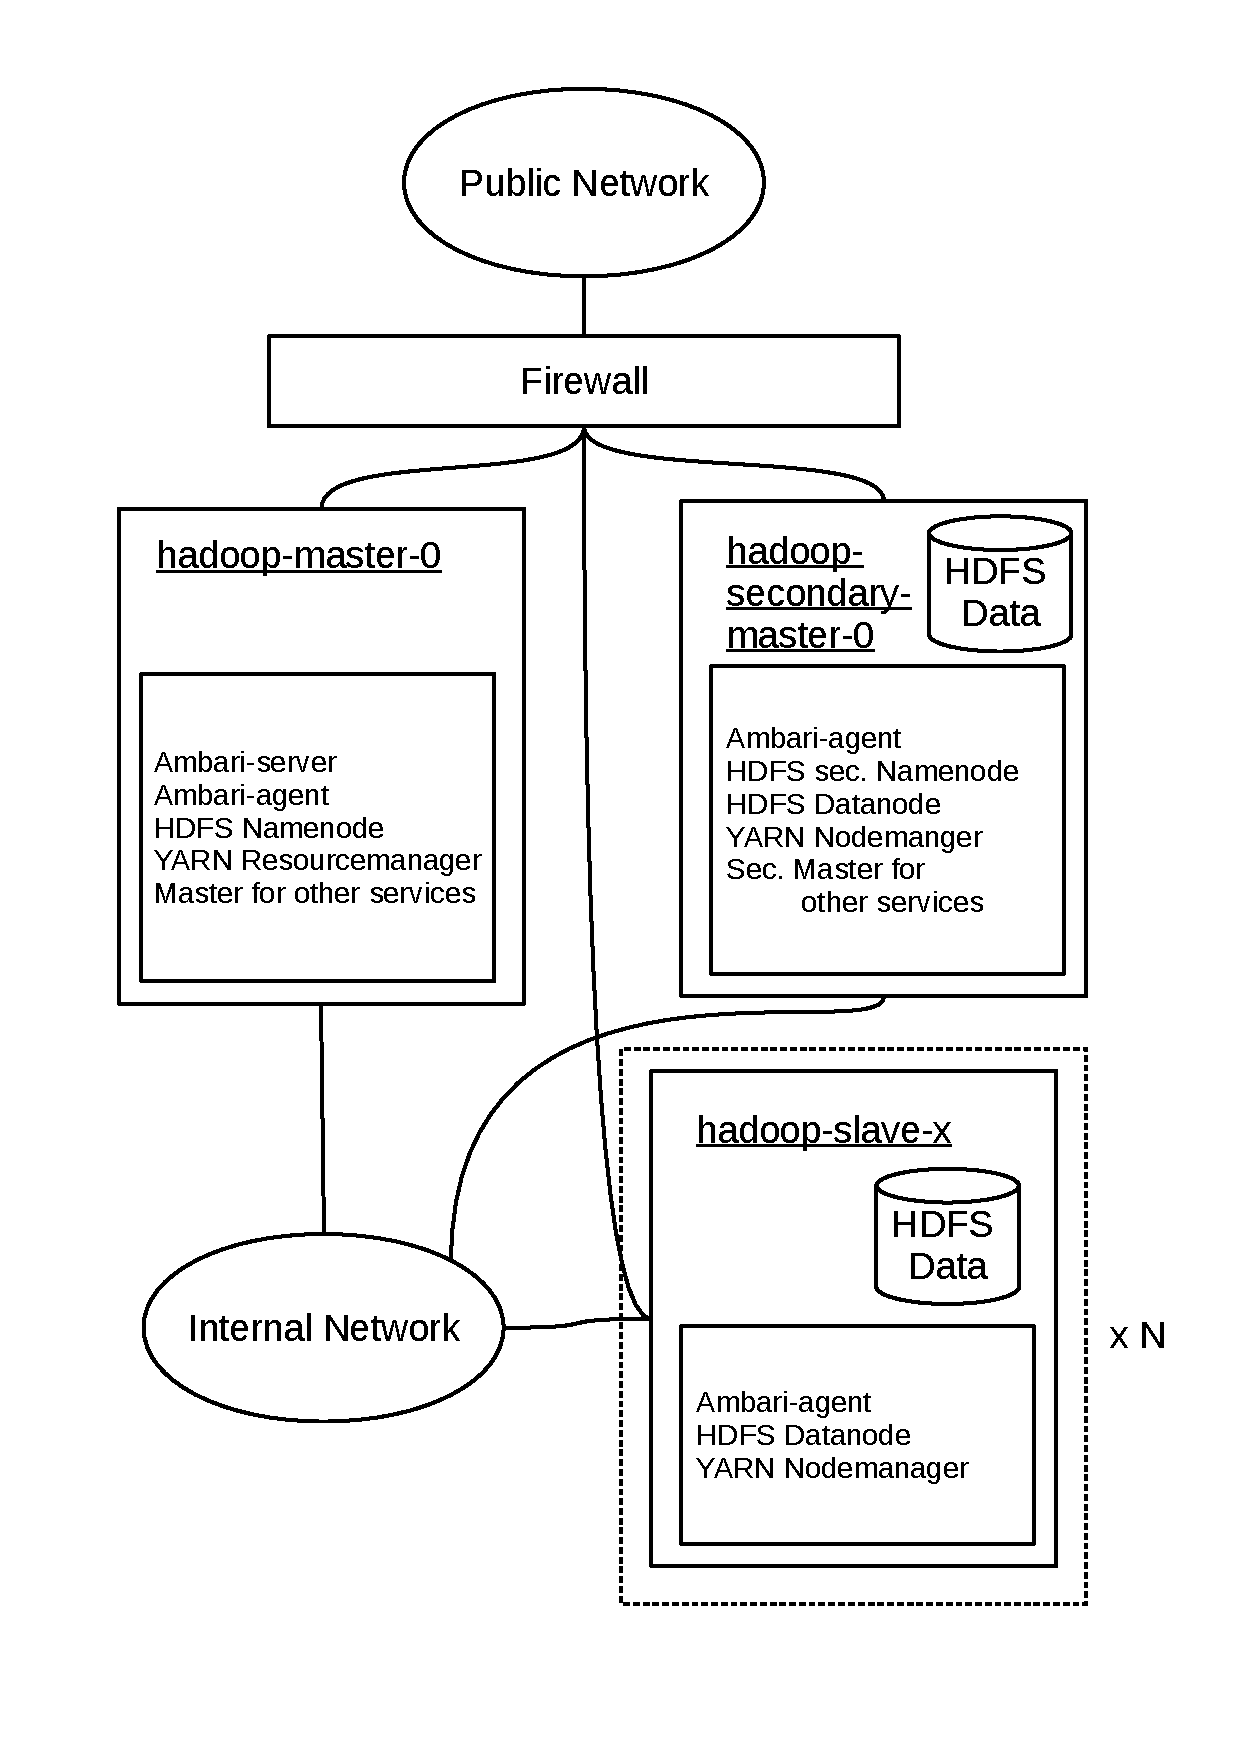
\includegraphics[width=\textwidth,height=\textheight,keepaspectratio]{resources/architecture.pdf}
    }
	\caption{\label{fig:architecture}Proposed Architecture}
\end{figure}

As discovered in section \vref{sec:ambari:errors} there should be at least 50 \ac{GB} of disk space on each node, 
just for Ambari and Hadoop to be installed.
For \ac{HDFS} data storage an additional volume should be attached to each of the \ac{HDFS} DataNodes.

The size of the used \acs{VM} should be the one with the most memory, 
as this is the resource where the overhead of having multiple \acs{VM} has the most impact.
All nodes need access to the Internet to download software packages and should be accessible via \ac{SSH} through the OpenStack firewall.
Furthermore the master node needs to be accessible via typical ports for the web interface of the deployed services and other ports which clients use to connect to the Hadoop cluster and issue jobs to it.
Internally all nodes need to be connected via an private network with fixed \acs{IP}, where the mapping between hostnames and \acs{IP} is known for each host. Typically this can be done with \ac{DNS}, however it is out of scope for this project to setup an \ac{DNS} server. Filling the \texttt{\/etc\/hosts} file is sufficient.
The internal network should not be restricted by any firewall.

Tom White recommends the following specification for a single node in a cluster, based on the needs of a full \ac{BDA} system in 2014:\\

\begin{itemize}
    \item Each node should run on dedicated, commodity hardware.
    \item Processor - Two hex/octo-core 3 GHz \acs{CPU}
    \item Memory 64 to 512 \ac{GB} \ac{ECC} \ac{RAM}
    \item Storage - 12 to 24 times 1 to 4 \ac{TB} disks
    \item Network - Gigabit Ethernet with link aggregation
\end{itemize}
\autocite{white2015hadoop}

However the given OpenStack environment does not allow the allocation of such amounts of resources, and has no possibility to use dedicated hardware. 
Therefore the maximum sized \acs{VM} should be used, and each be given an equal share of the available storage.

In case that it is only possible to allocate a small number of \acp{VM}, it can be useful to also assign the role of a DataNode and NodeManager to the master node. This allows the available resources on the master node not only to be used for management purposes but also for processing.

\section{Execution Plan}

In chapter \ref{chap:impl} the Hadoop cluster will be set up in an automated way.
To do so an execution plan is provided.
It functions as a reference to follow along during the implementation 
and can be used to reproduce the results in a similar way, i.e. to set up the cluster again in an similar environment.

In section \vref{sec:decision} the decision to use Apache Ambari in combination with Ansible has been made.
This scenario leads to the following steps regarding the deployment of the cluster into the OpenStack environment:

\begin{enumerate}
    \item \textbf{\ac{VM} Creation in OpenStack}
    As the first step, the host \acp{VM} need to be created in the OpenStack environment which will form the cluster.
    \begin{enumerate}
        \item Create an internal network.
        \item Create security groups which allow access with \ac{SSH}) to the hosts and via the web management portal to Ambari.
        \item Create an appropriate number of maximum sized \acp{VM} that are connected to both the internal and external network. Name them according to the names in \ref{fig:architecture}. Use a common domain, even if it is not officially registered. Provide some SSH credentials to log in.
        Assign the previously created security group to them.
        Ubuntu 14.04 or 16.04 should be used as the operating system.
        \item Note down the assigned internal and external \ac{IP} addresses displayed by OpenStack.
        \item Create virtual disks and assign them to the nodes. They will be used to store \ac{HDFS} data on them.
    \end{enumerate}
    
    \item \textbf{System Set-Up with Ansible} 
    In section \vref{sec:design:hdp_ambari_ansible} it has been shown that Ansible can be used to deploy \ac{HDP}. The Ansible playbook developed for this purpose can be adapted and used in the next steps.
    \begin{enumerate}
        %\item Configure the \texttt{ssh\_config} configuration file by supplying the \acp{FQDN} and the public \ac{IP} addresses of the nodes. 
        \item Configure the local \ac{SSH} client to use the \acp{FQDN} and the public \ac{IP} addresses of the nodes. 
        \item Check that all nodes can actually be accessed via \ac{SSH}
        \item Note down the name of the secondary (internal) Ethernet adapter of each node.
        \item Configure the Ansible inventory. Supply the internal \ac{IP} address as well as the previously noted Ethernet adapter of the node. he \emph{hadoop-master-0} node should be listed in the \emph{master} section, all others in the \emph{slave} section.
        \item Prepare the nodes for the usage with Ansible by installing Python on them and upgrading all system packages.
        \item Apply the Ansible playbook to the hosts.
        This configures the host systems in such a way that Ambari Server and Client respectively are installed on them.
    \end{enumerate}
    
    \item \textbf{Hadoop Set-Up with Ambari} 
    Next Hadoop itself, together with additional tools, can be deployed to the cluster using the Ambari cluster installation dialogue. This follows the instructions from \autocite[][Chap.~6]{hortonworks2018install}
    
    \begin{enumerate}
        \item Connect to Ambari via the web interface on the master node. The complete installation can be done from there.
        \item Ambari offers an cluster installation dialogue that firsts asks for all necessary configuration and checks it for consistency. The dialogue's instructions can be followed to deploy a cluster. 
        \item To select the hosts that should be included in the cluster, the \acp{FQDN} including a domain extension of all the \acp{VM} that have been created in the previous step should be provided.
        \item The \enquote{manual registration} option should be chosen, since otherwise an non-encrypted \ac{SSH} private key must be uploaded, which is unsafe.
        \item Next select the services and tools that should be included in the cluster installation. Hadoop is clearly mandatory, other tools that should be included are listed in \emph{Jonas Balsfullands' paper}. If Ambari detects unmet inter-dependencies, those should be corrected. 
        \item Assign the \emph{master} host to inhabit the master role in each service. If the service offers the possibility to register a secondary, fallback master this should be assigned to the \emph{secondary master} host.
        \item Assign slave nodes and clients to all of the nodes. This includes \emph{DataNodes} and \emph{NodeManager} and the Hadoop client tools.
        \item Configure all the services to the needs for the cluster. Most default settings can be kept. No service should depend on external resources such as existing databases. Set passwords to the services where needed. The passwords that have been set for each individual service should be documented. Ambari checks the settings for soundness and possibly warnings can be resolved manually.
        \item The installation then is being performed on the cluster. All selected components are installed with the selected configuration.
    \end{enumerate}
    
    \item \textbf{Test Usage} 
        To verify that the previous steps were successful, it is necessary to tests that the Hadoop cluster can be used
        \begin{enumerate}
            %\item Test that the master node can be reached from within the \ac{DHBW} network by connecting to it with a \ac{} and 
            
            % test connection to Hadoop master with hadoop client installed on workstation
            \item Test that \ac{HDFS} works by storing multiple, different sized files on the cluster file system.
            \item Test that MapReduce can be used to process data by running \emph{teragen} and \emph{terasort} on the cluster to create different amount of numbers and sort them. For example datasets with 100~\ac{MB}, 1~\ac{GB} and 5~\ac{GB} can be used for the tests.
        \end{enumerate}

\end{enumerate}

In the next chapter this execution plan will be implemented. More details about the technical solution and the exact execution, as well as the Ansible playbook will be given.



% !TEX root = ../master.tex
\chapter{Implementation}
\label{chap:impl}

The previous chapter yielded a general execution plan that shall implemented in the coming 
section while utilizing the cluster computer at the \ac{DHBW}. 
For each implementation detail the specifically chosen values are given during the process. Each of the steps holds 
the possibilities for errors which will also be evaluated.
The outcome of the taken steps is only a partially functional Hadoop cluster.
The reasons and implications for this restricted outcome are given.
Suggestions for future projects how better results might be achieved is given in the end.

\section{Infrastructure Set-Up in OpenStack}

\subsection{Preparation}

The foundation for the cluster architecture that has been illustrated in figure \vref{fig:architecture} are the host \acp{VM}, their storage and the network that connects them.
In the course of this process some minor adaptions are made to the proposed architecture.
Especially the \texttt{hadoop-master-0} node now also runs the \ac{HDFS} DataNode and YARN NodeManager service and therefore has a storage volume attached to it.

To set up the cluster the web interface of OpenStack can be used, which is accessible at
\urlinline{https://controller.c4.dhbw-mannheim.de/} from within the \ac{DHBW} network.
Each operation on the infrastructure can be performed within this interface.

\subsection{Execution}

\subsubsection{Firewall Rules}

The firewall in OpenStack can be configured by creating \emph{security groups}.
These security groups describe rules for allowing and prohibit outgoing and incoming connections.
For this project two security groups are created and assigned to each of the \acp{VM}.
The first group deals with \emph{default} settings. It allows all outgoing connections 
and allows incoming connections on port 22, which is the port used for \ac{SSH} access, 
as well as incoming ping packages in the Internet Control Message Protocol.
The second group deals with Hadoop specific ports.
A detailed over all necessary ports is given by \textcite{hortonworks2017reference} in their port reference.
However to make development and access more flexible, this group does temporarily 
allow all incoming requests.

\subsubsection{Network}

To enable an interconnection between the nodes in the cluster it is useful to create a private network between them.
The network uses the address space of 10.100.10.0/24 which is a sub-network of the private address space defined in RFC~1918 by the the Internet Engineering Task Force \autocite[][]{ietf1996rfc1918}.
Figure \ref{fig:networks_subnets} lists all the networks that are available after the internal network is created. 
The network named \emph{int-net-10} is the internal network which all nodes connect to. Furthermore all nodes need to connect to the \emph{ext-net-201} network which allows them to connect to the Internet and makes them accessible from within the \ac{DHBW} network.

\begin{table}[hbt]
\resizebox{\textwidth}{!}{%
	\begin{tabular}{lll}
	  Network Name & Sub-networks & Description\\
	  \hline
	  ext-net-201 & 141.72.191.0/24 & Pre-configured connection to \ac{DHBW} internal network\\
	  ext-net-112 & 192.168.112.0/20 & Pre-configured connection with unknown connectivity\\
	  int-net-10 & 10.100.10.0/24 &  New internal network used by Hadoop\\
	\end{tabular}%
	}
	\caption{Sub-networks within the project in OpenStack}
	\label{fig:networks_subnets}
\end{table}

\begin{figure}[hbt]
  {\centering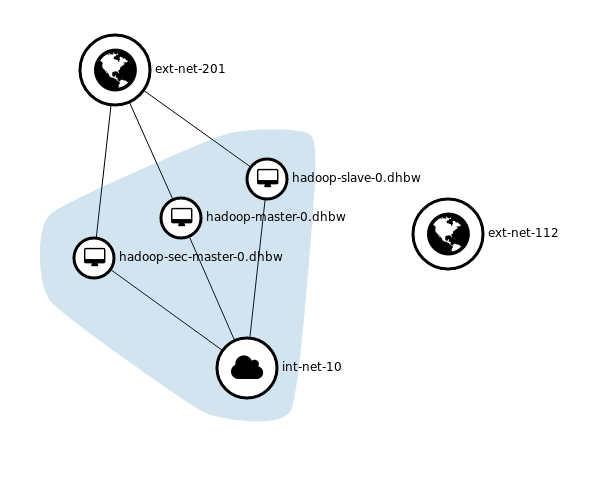
\includegraphics[width=0.8\textwidth]{{img/network_topology}.png}\par}
  \caption{Network topology created in OpenStack}
  \label{fig:network_topology}
\end{figure}

Once the nodes are created, the network topology looks like figure \ref{fig:network_topology}. The highlighted denotes the network connections that exists purely in OpenStack and have no physical connection to any outside network.
The figure also shows the names of the hosts and the network names.

\subsubsection{Virtual Machines}

In the next step the virtual machines are created.
The OpenStack environment offers different \emph{flavors} of instance sized for the \acp{VM} which is a pre-configured combination of resources associated to it.
To create a node the developer can chose from the presets listed in table \ref{fig:instance_sizes}. The flavors differ in amount of \acp{VCPU}, \ac{RAM} and root storage.
The set-up of the hosts is done for each node individually, 
since the names and flavor configurations differ between them.
The names are respective to proposed architecture but have a \emph{dhbw} domain ending 
added to them, which is not officially registered but is necessary for Ambari to identify the hosts correctly.


\begin{table}[hbt]
\centering
\resizebox{0.8\textwidth}{!}{%
	\begin{tabular}{lrrr}
	  Instance Flavor Name & \acp{VCPU} & \acs{RAM} & Root Disk Size \\
	  \hline
	  m1.nano & 1 & 64~\acs{MB} & 1~\acs{GB} \\
	  m1.tiny & 1 & 512~\acs{MB} & 5~\acs{GB} \\
	  m1.small & 1 & 1~\acs{GB} & 10~\acs{GB} \\
	  m1.medium & 2 & 2~\acs{GB} & 20~\acs{GB} \\
	  m1.large & 4 & 4~\acs{GB} & 40~\acs{GB} \\
	  m1.xlarge & 8 & 8~\acs{GB} & 80~\acs{GB} \\
	\end{tabular}%
	}
	\caption{Available instance sizes in the \ac{DHBW} OpenStack environment}
	\label{fig:instance_sizes}
\end{table}


\begin{table}[hbt]
\centering
	\begin{tabular}{lrl}
	  Resource Type & Amount & Unit\\
	  \hline
	  Instances & 10 & \\
	  \acp{VCPU} & 20 & \\
	  \acs{RAM} & 51200 & \acs{MB} \\
	  Floating \acs{IP} Addresses & 10 & \\
	  Security Groups & 10 & \\
	  Volumes & 10 & \\
	  Volume Storage & 1000 & \acs{GB}
	\end{tabular}
	\caption{Available resources for the project in the \ac{DHBW} OpenStack environment}
	\label{fig:resources_openstack}
\end{table}

Table \ref{fig:resources_openstack} describes how many resources are available at maximum for the project in the \ac{DHBW} OpenStack environment. The chosen configurations may in sum not exceed this limit.
As visible in table \ref{fig:instance_sizes} all instance of m1.small and larger have a core to memory ration of \emph{1~core~:~1~GB~RAM}, which means that, if all 20 available cores are used, only 20 out of 51.2 GB RAM  can be used. It is favourable to have maximum sized \acp{VM} with respect to memory to give Hadoop the possibility make better use of it.
Therefore the best allocation for the nodes is to use a m1.xlarge instance for the master node, a m1.xlarge for the secondary and a large instance for the slave node.
This in sum gives 20 \acp{VCPU} and 20~\ac{GB} \ac{RAM} and no further cores are available to allocate more nodes.


Each instance is using the Ubuntu 16.04 operating system which is compatible with \ac{HDP}, Ambari and Hadoop. As discussed before the security groups for default access and Hadoop specific access are assigned to the hosts, and they are connected to the internal and external network. An \ac{SSH} key is used for authentication.
The successful creation of each host is tested by accessing it via \ac{SSH} using the specified key and the user \emph{ubuntu}.


\subsubsection{Storage}

In order for the Hadoop cluster to store \ac{HDFS} data it is necessary to split up the available 1000~\ac{GB} for storage into three volumes, one for each host.
The disks are attached to the hosts and OpenStack reports the device handle that can be 
used within the hosts to access the volume.
Before data can be stored on the volumes they each need to be partitioned into one partition using the program \texttt{fdisk}. The partitions are then formatted into ext4 file system format using the \texttt{mkfs.ext4} command.

\subsection{Encountered Issues and Lessons Learned}

Access to the OpenStack environment and the cluster nodes is only possible from within the \ac{DHBW} network that connects the \ac{DHBW} Mannheim and Stuttgart.
This network is not accessible via an virtual private network and the developer needs to be on premise of the \ac{DHBW}. This restriction in locality makes the development process harder.

During the implementation, the OpenStack environment showed significant instabilities.
\emph{Internal errors} lead in some cases to the failure of allocation of resources for the requested \acp{VM}.
This might indicate an general shortage of resources in the \ac{DHBW} OpenStack environment. Later in the project these internal errors have been resolved.

\section{System Set-Up with Ansible}

As laid out in the evaluation of Ambari in section \vref{sec:design:hdp_ambari_ansible} 
and the execution plan, 
an Ansible playbook that was developed for the evaluation is now adapted to perform the system setup of the cluster. 
The next section will discuss the how this playbook is structured and what actions are performed to install the system.
The full Ansible playbook including all roles and templates is stored on the authors \emph{GitHub repository} and can be accessed at 
\urlinline{https://github.com/XOSplicer/studienarbeit-hadoop-cluster-ansible}.
The important excerpts, which are the \emph{task definitions}, are also attached in the appendix \vref{app:ansible}.

\subsection{Preparation}

Before Ansible can be used by the developer, it needs to be installed locally.

TODO also install Ansible locally
TODO explain and maybe print this particular playbook yes yes print it with explanations
TODO maybe appendix

TODO describe all roles and task within those roles

TODO \vref{lst:ansibleall}

\subsubsection{Common Set-Up Tasks}
TODO \vref{lst:ansiblecommon}

\begin{enumerate}
    \item TODO set the hostname
    \item TODO configure the host file for local resulution
    \item TODO make sure the correct ssh keys can be used for access
    \item TODO install common necessary packages (which? and why, see install manual aswell)
    \item TODO install and activate ntp
    \item TODO configure internal network, apply if necessary
    \item TODO register the ambari repository list inluding keys and load their contents
    \item TODO disblae the thp feature using a service
    
\end{enumerate}

\subsubsection{Specific Tasks for Ambari Server}
TODO \vref{lst:ansiblemaster}

\begin{enumerate}
    \item TODO install the ambari server package
    \item TODO setup the ambari server
    \item TODO activate the server service if not yet running
\end{enumerate}

\subsubsection{Specific Tasks for Ambari Client}
TODO \vref{lst:ansibleslave}

\begin{enumerate}
    \item TODO mount the storage volume
    \item TODO install ambari agent
    \item TODO configure ambari agent to use masternode as master hostname
    \item TODO restart or start the service if necessary
\end{enumerate}

\subsection{Execution}

In order to configure the hosts with Ansible they must be accessible via \ac{SSH} by their \ac{FQDN}. 
Since no \ac{DNS} system is employed, the \texttt{ssh\_config} file is used to provide a local resolution for \ac{SSH}. 
Listing \ref{lst:sshconfig} describes how this configuration looks like.

\lstset{language=sh}
\begin{lstlisting}[caption={Local SSH configuration file used by Ansible}, label={lst:sshconfig}]
Host hadoop-master-0.dhbw
    Hostname 141.72.191.54
    user ubuntu

Host hadoop-sec-master-0.dhbw
    Hostname 141.72.191.55
    user ubuntu

Host hadoop-slave-0.dhbw
    Hostname 141.72.191.56
    user ubuntu
\end{lstlisting}

Before a host can be used with Ansible, it needs to have \emph{Python 2} installed.
Therefore a short script cat be run on each host, which updates the system, installs Python and reboots the system. This ensures all packages are up to date. The following bash script performs these tasks and also installs the \emph{python-apt} library which is necessary for Ansible to install more packages.

\lstset{language=sh}
\begin{lstlisting}[caption={Bash script for initial host preparation}, label={lst:hostsetup}]
sudo apt-get update \&\& sudo apt-get -y upgrade
sudo apt-get -y install python2.7 python-apt
sudo reboot now
\end{lstlisting}

After this initial preparation of the hosts is done, 
the Ansible inventory can is configured, 
so that all the specific variables of the host are set. 
These variables are the \ac{FQDN}, the internal \ac{IP} address, 
the network interface that is connected to the internal network 
and finally the \ac{UUID} of the partition that is used to store the \ac{HDFS} data.

The \ac{FQDN} is again taken from the \texttt{ssh\_config} file. 
The internal \ac{IP} address is taken from the OpenStack web interface.
To find the values for the other variables each host is accessed.
The internal network interface is the second Ethernet interface listed with the command \texttt{\$ ifconfig -a}. Typically it is called \texttt{ens4}, \texttt{ens6} or \texttt{ens7}.
The \ac{UUID} of the storage volume is found by running \texttt{\$ sudo blkid}. 
It reports the \ac{UUID} of all volumes. The one corresponding to the device that has been created in OpenStack can be found in the output. These variables are then entered into the \texttt{inventory.ini} file for Ansible. The master node is entered in the \texttt{master} section, the slave nodes in the \texttt{slave section respectively}.

\lstset{language=sh}
\begin{lstlisting}[caption={Exemplary inventory description in Ansible}, label={lst:inventory}]
[master]
hadoop-master-0.dhbw internal_ip=10.100.10.24 iface_internal=ens4 hadoop_vol_uuid=47103a5e-5c3f-40f3-a710-fcd86e23fc61

[slave]
hadoop-sec-master-0.dhbw internal_ip=10.100.10.25 iface_internal=ens4 hadoop_vol_uuid=54b1d167-9b88-45c1-b27f-6e441b765c66
hadoop-slave-0.dhbw internal_ip=10.100.10.26 iface_internal=ens4 hadoop_vol_uuid=046a2bc2-df33-4640-becd-2c401076285f
\end{lstlisting}

Now all necessary variables are set and the Ansible playbook is be applied to the hosts.
This is done using the command \texttt{\$ ansible-playbook all}.
Ansible connects to each of the hosts and performs the necessary steps to get the system into the desired state.

\subsection{Encountered Issues and Lessons Learned}

Ansible proved very capable to perform system administration tasks in a reproducible fashion. 
It has extensive documentation that describe how a given configuration can be expressed in an Ansible playbook. 
Therefore it is suited to describe \enquote{system configuration as code} in an complexity that can be handled with reasonable effort.

\section{Hadoop Set-Up with Ambari}

\subsection{Preparation}

After the Ambari software is installed on each host by Ansible, it can be utilized to set-up the Hadoop cluster and install additional tools as well.
To do so the Ambari web interface is used that can be accessed on the master node on port 8080. The complete Hadoop setup is performed using the cluster deployment dialogue that Ambari offers. This process follows the execution plan closely.

\emph{Jonas Balsfulland} proposes in his paper which additional tools should be running on the cluster. Especially \emph{Spark 2, Storm, Hive and Pig} should be deployed.
Ambari offers the possibility to set up all of these services automatically if they are selected during the cluster setup.

\subsection{Execution}

The deployment dialogue in Ambari guides the user through the cluster installation.
For this project a cluster named \emph{hadoopdhbw0} is created which installs \ac{HDP} Version 2.6.3.0. All binary packages are downloaded from Hortonworks repositories.
The list of the \acp{FQDN} including the \emph{dhbw} domain of the three \acp{VM} are entered as cluster nodes. They are registered using \emph{manual registration} since the Ambari agent installed on all nodes is configured to contact the master node as the Ambari server. Furthermore this elides the necessity to upload an unencrypted \ac{SSH} key with root access to the servers.
Ambari then checks the connectivity to each host and performs preliminary checks about the host that ensure the cluster can be deployed successfully.

Next the services and additional tools are chosen which are installed on the cluster.
For this setup \ac{HDFS}, \ac{YARN}, MapReduce2, Tez, Hive, Pig, ZooKeeper, Storm, SmartSense, Spark2, Slider and Ambari Metrics are selected. SmartSense, Slider, ZooKeeper and Ambari Metrics are enforced to be installed by Ambari. 
After this Ambari lets the user configure which master, slave and client components of each service are placed on each host.
Obviously all master components are placed on the master host, while the slave components are installed on all all hosts.
Finally each service is configured specifically. 
Ambari provides preset for each service.
Those presets provide a basic configuration that is sufficient for the purpose of this project. 
The only preferences which are made are the passwords.

In the end Ambari deploys the Hadoop cluster by installing the components in the requested 
configuration. 
This process is automatic and when it is finished Ambari tries to start up the cluster components. The user then is redirected to the Ambari service overview in the web interface where the status of each service is monitored and the services can be managed while the cluster is running. This includes starting and stopping the service, as well as re-configuring it.

\subsection{Encountered Issues and Lessons Learned}

During the initial evaluation of Ambari in section \vref{sec:design:hdp_ambari_ansible} it was figured that 20~\ac{GB} of root storage for the installation of the cluster is not enough. This approach uses a reduced set of services that are installed which leads to less disk space needed. Therefore the 80~\ac{GB} root volume is sufficient on all nodes as expected previously.

During the installation process in Ambari several issues regarding domain name resolution appeared.
This is caused by the fact that no proper \ac{DNS} server is used to distribute the \acp{FQDN} 
but rather the \texttt{hosts} file is altered in a way that the resolution works locally between all nodes. 
This holds the possibility for configuration errors which lead which lead to the failure of the installation at first.
The issues are fixed by adapting the \texttt{hosts} file to only perform name resolution for the selected \acp{FQDN} for the local, internal network. 

One major issue is encountered when Ambari tries to start all services: The main memory on the master node, which is limited to 8~\ac{GB} is not sufficient and the system is instable.
When the master node runs out of memory the operating system can kill arbitrary services that are running
Since this is happening on the master node, this leads to the service not being available at all and introduces the need for manual restarting of the service.
In conclusion some services are turned of explicitly to improve stability. 
In particular Hive, SmartSense and Spark2 are deactivated for the entire cluster. 
This way the master node has enough memory to run the other services.

\section{System Tests}

Before the processing system can be tested a new directory to store the test data in \ac{HDFS}
is created. 
This folder is \texttt{/user/ubuntu} and is accessible by the user \texttt{ubuntu}.
To test this step a new file is uploaded to the directory and its content is then downloaded again which tests successful. The directory is used in the next step.

\subsubsection{Terasort}

As suggested in the execution plan the \emph{terasort} program implemented by \textcite{omally2008terasort}, which is included in the Hadoop installation on each cluster node, is used to check the sanity of the \ac{YARN}, \ac{HDFS} and MapReduce2 Services.
First \emph{teragen} generates a variable amount of random numbers and stores them on \ac{HDFS}. Then \emph{terasort} sorts the numbers using MapReduce and stores the result.
Finally \emph{teravalidate} checks that the numbers are indeed sorted correctly.
To run the test the following commands are used to create 5~\ac{GB} fo data:

\lstset{language=sh}
\begin{lstlisting}[caption={Running Terasort as a test for YARN and HDFS}, label={lst:terasort}]
hadoop jar hadoop-mapreduce-examples.jar teragen 5000000 /user/ubuntu/test/5gsort/input
hadoop jar hadoop-mapreduce-examples.jar terasort /user/ubuntu/test/5gsort/input /user/ubuntu/test/5gsort/output
hadoop jar hadoop-mapreduce-examples.jar teravalidate /user/ubuntu/test/5gsort/output
\end{lstlisting}

The test are done for 1~\ac{MB}, 1~\ac{GB} and 5~\ac{GB}.
All test finish successfully, which means that MapReduce jobs can be successfully scheduled on the cluster and can interact with \ac{HDFS}.

\subsubsection{Ambari Service Checks}

Ambari offers the possibility to run \emph{service checks}, which run a small workload on one service and makes sure the cluster behaves correctly.
These checks are run in this project for all services that are active.
The services that are inactive due to memory shortage can not be tested.
The checks are therefore performed  only for \ac{HDFS}, \ac{YARN}, MapReduce2, ZooKeeper, Storm, and Ambari Metrics. All of the checks are giving successful results, which only means the service works as expected. It does not show that all nodes are participating in the cluster for this service. 

\section{Conclusion}

In general the cluster installation is only partially successful since the services are not running reliably and some even are not active at all due to memory limitations.
The produced cluster is therefore not ready for \emph{production use}.
However the general concept of using OpenStack to host the cluster and Ansible and Ambari to deploy the cluster software and manage Hadoop is possible and has clearly advantages above a manual cluster management.

During the project the \ac{DHBW} Cloud environment showed unreliabilities that influenced the progress of the implementation phase.
The general process was errorsome and would be hard to reproduce for students or lecturers with little knowledge about system administration. It is therefore not recommended to pursue a installation of Hadoop within the context of a lecture. 

In future projects a master node with significantly more resources should be used 
if the project uses the OpenStack environment at the \ac{DHBW}.
This however requires new flavors for instance sizes which have more memory in respect to the processing cores.
An alternative would be to use dedicated servers within the \ac{DHBW} or to 
get a contract with a \emph{managed platform} vendor who provides Hadoop as a service.


% !TEX root = ../master.tex
\chapter{Conclusions}
\lipsum

%	Literaturverzeichnis
\ihead{} % Neue Header-Definition
\printbibliography

%\printglossaries

%----------------------------------------
% Anhang
% Hier können alle Anhänge als einzelne Datei eingefügt werden.
% Die Anhänge werden gesondert alphabethisch benannt (A Anhang 1, B Anhang 2, usw)
%----------------------------------------
\appendix
\ihead{\appendixname~\thechapter} % Neue Header-Definition

% !TEX root = ../master.tex

\chapter{Appendix A - Ansible Playbook Descriptions}

\lstset{language=sh}
\begin{lstlisting}[caption={Ansible playbook that gets run to install the cluster system}, label={lst:allplaybook}]
---
- hosts: master
  roles:
    - role: master
      become: true
    - role: slave
      become: true

- hosts: slave
  roles:
    - role: slave
become: true
\end{lstlisting}

\lstset{language=sh}
\begin{lstlisting}[caption={Common tasks in Ansible}, label={lst:commontasks}]
- name: Set hostname
  hostname: name="{{ inventory_hostname }}"

- name: Set /etc/hosts
  template:
    src: "{{ role_path }}/templates/hosts.j2"
    dest: /etc/hosts
    owner: root
    group: root
    mode: 0644
    backup: yes

- name: Set authorized_keys for user ubuntu
  copy:
    src: "{{ role_path }}/files/authorized_keys"
    dest: /home/ubuntu/.ssh/authorized_keys
    owner: ubuntu
    group: ubuntu
    mode: 0600
    backup: yes

- name: Install common packages
  apt: pkg="{{ item }}" state=installed update_cache=true
  with_items:
    - "{{ pkg_pycurl }}"
    - "{{ pkg_curl }}"
    - "{{ pkg_unzip }}"
    - "{{ pkg_tar }}"
    - "{{ pkg_wget }}"

- name: Install ntp
  apt: pkg={{ pkg_ntp }} state=installed update_cache=true

- name: Activate ntp service
  service:
    name: ntp
    enabled: yes
    state: started

- name: Set interfaces file to load all interfaces in interfaces.d
  copy:
    src: "{{ role_path }}/files/interfaces"
    dest: /etc/network/interfaces
    owner: root
    group: root
    mode: 0644
    backup: yes

- name: Set internal network config
  template:
    src: "{{ role_path }}/templates/60-internal.cfg.j2"
    dest: /etc/network/interfaces.d/60-internal.cfg
    owner: root
    group: root
    mode: 0644
    backup: yes
  register: if_internal_restart

- name: Restart internal network interface
  shell: "ifdown {{ iface_internal }} && ifup {{ iface_internal }}"
  when: if_internal_restart | changed

- name: Download Ambari repository list
  get_url:
    url: "{{ ambari_repo_list }}"
    dest: /etc/apt/sources.list.d/ambari.list
    mode: 0644
    backup: yes

- name: Add Ambari repository key
  apt_key:
    keyserver: "{{ ambari_repo_keyserver }}"
    id: "{{ ambari_repo_keyid }}"

- name: Update apt cache
  apt:
    update_cache: yes

- name: Copy transparent-huge-pages service file
  copy:
    src: disable-transparent-hugepages
    dest: "/etc/init.d/disable-transparent-hugepages"
    mode: 0755

- name: Run service to disable transparent hugepages
  service:
    name: disable-transparent-hugepages
    state: started
enabled: yes
\end{lstlisting}


\lstset{language=sh}
\begin{lstlisting}[caption={Ansible playbook that gets run to install the cluster system}, label={lst:allplaybook}]
---
- hosts: master
  roles:
    - role: master
      become: true
    - role: slave
      become: true

- hosts: slave
  roles:
    - role: slave
become: true
\end{lstlisting}


\end{document}
